\section{Mesure de performance}

Je profite de ce rapport pour parler d'un travail qui m'a été demandé en entreprise. Nous utilisons le framework EO\footnote{Evolving Object, \url{http://eodev.sf.net}} pour développer nos algorithmes évolutionnaires\footnote{Algorithme évolutionnaire : \url{http://fr.wikipedia.org/wiki/Algorithme_evolutionnaire}}. Le sujet consistait à implémenter, au framework EO, un parallélisme à mémoire partagée en utilisant OpenMP.

\subsection{Préambule}

Avant de commencer il est important de préciser que les EA\footnote{Algorithmes évolutionnaires} travaillent sur une population d'individu aussi appelé échantillon. Un individu étant représenté par un point dans l'échantillon, la complexité d'un problème est définit par le nombre de dimensions pour chaque individu.\\

Le problème est représenté par la fonction objectif qui prend en paramètre un individu (un point dans l'échantillon) et évalue toutes ses dimensions pour en déduire la qualité\footnote{Fitness en anglais}. La qualité est le critère de comparaison d'un point dans son échantillon.

\subsection{Identifier les ressources les plus utilisées}

Un test de profiling a été exécuté afin d'identifier les ressources les plus utilisées dans le framework EO. Le test nous a permit d'identifier une fonction qui est utilisée par une grande majorité des opérateurs\footnote{Opérateurs de sélection et variation} EO. Il s'agit de la fonction ``apply''. Elle prend en paramètres une population d'individu et un opérateur. Cette fonction va itérer sur tous les individus de la population et appliquer l'opérateur. Il peut être intéressant d'optimiser cette fonction. Nous allons nous limiter à transformer le code séquentiel en parallèle.

\subsection{Pseudo-code de la fonction apply}

L'algorithme \ref{apply} prend en paramètre une population ainsi qu'un opérateur à appliquer à chaque individu.

\incmargin{1em}
\begin{algorithm}[here]
  \dontprintsemicolon
  \Donnees{$P \in K_n, F \in Operateur$}
  \Res{$B' \in K_n$}
  \Deb{
    \Pour{$i\leftarrow 0$ \KwA $n$}{
      $F(P(i))$
    }
  }
  \caption{La fonction apply}
  \label{apply}
\end{algorithm}
\decmargin{1em}

\subsection{La fonction en parallèle}

L'algorithme \ref{omp_apply} transforme la fonction ``apply'' en parallèle en utilisant le modèle PRAM CREW\footnote{Concurantial Read Exclusive Write} et $O(n)$ processeurs pour parcourir tous les individus de la population.

\incmargin{1em}
\begin{algorithm}[here]
  \dontprintsemicolon
  \Donnees{$P \in K_n, F \in Operateur$}
  \Res{$B' \in K_n$}
  \Deb{
    \textit{parallèle}\;
    \Pour{$i\leftarrow 0$ \KwA $n$}{
      $F(P(i))$
    }
  }
  \caption{La fonction omp\_apply}
  \label{omp_apply}
\end{algorithm}
\decmargin{1em}

\subsection{Speed-up}

Après avoir crée la fonction alternative employant le parallélisme à mémoire partagée, appelé ``omp\_apply'', nous allons étudier une solution de mesure du speed-up\footnote{$S_p = \frac{T_1^*}{T_p}$ : \url{http ://en.wikipedia.org/wiki/Speedup}}.\\

L'équation, en figure \ref{fig:mesure_speedup}, présente une méthode de mesure du speed-up et est implémentée dans l'algorithme \ref{algo_speedup}.

\begin{figure}[here]
\centering
$$Mesure\ du\ Speedup = r \sum^{P,D}_{k=0,l=0} S_{p_{kl}}$$
\caption{Mesure du Speedup}
\label{fig:mesure_speedup}
\end{figure}

\incmargin{1em}
\begin{algorithm}[here]
  \dontprintsemicolon
  \Donnees{$p, P, popStep, d, D, dimStep, r \in N$}
  \Deb{
    \Pour{$k\leftarrow p$ \KwA $P$}{
      \Pour{$l\leftarrow d$ \KwA $D$}{
        \Pour{$m\leftarrow 0$ \KwA $r$}{
          $T_s\leftarrow 0$\;
          $T_p\leftarrow 0$\;
          \Deb{
            $t_1\leftarrow omp\_get\_wtime()$\;
            ... code sequentiel avec $k$ et $l$ exécuté $m$ fois ...\;
            apply( ... )\;
            $t_2\leftarrow omp\_get\_wtime()$\;
            $T_s\leftarrow t_2 - t_1$\;
          }
          \Deb{
            $t_1\leftarrow omp\_get\_wtime()$\;
            ... code parallèle avec $k$ et $l$ exécuté $m$ fois ...\;
            omp\_apply( ... )\;
            $t_2\leftarrow omp\_get\_wtime()$\;
            $T_p\leftarrow t_2 - t_1$\;
          }
          ... on conserve le speed-up $\frac{T_s}{T_p}$ pour $k$ et $l$ ...\;
        }
      }
    }
  }
  \caption{La fonction de mesure du speedup}
  \label{algo_speedup}
\end{algorithm}
\decmargin{1em}

Une description des paramètres est disponible dans la figure \ref{fig:description_parametres}.

\begin{figure}[here]
  \centering
  \begin{tabular}{ | l | p{7cm} |}
    \hline
    \textbf{Paramètres} & \textbf{Description}\\\hline
    $p$ & la taille minimum de la population\\\hline
    $popStep$ & le pas d'iteration de la population\\\hline
    $P$ & la taille maximum de la population\\\hline
    $d$ & la taille minimum de la dimension\\\hline
    $dimStep$ & le pas d'iteration de la dimension\\\hline
    $D$ & la taille maximum de la dimension\\\hline
    $r$ & le nombre d'exécution pour chaque combinaison de $p$ et $d$\\\hline
  \end{tabular}
  \caption{Description des paramètres utilisés}
  \label{fig:description_parametres}
\end{figure}

\subsection{Mesures}

En prenant en compte les paramètres décrits précédemment, nous allons lancer les tests sur deux architectures matérielles différentes présenté en figure \ref{fig:architectures}.\\

\begin{figure}[here]
  \centering
  \begin{tabular}{ | l | l | l | l |}
    \hline
    \textbf{Processeur} & \textbf{Nombre de coeurs} & \textbf{Fréquence} & \textbf{Cache L1}\\\hline
    Intel Centrino vPro & 2 & 2.40GHz & 3072KB\\\hline
    Intel Core i7 & 8 (hyperthreading\footnote{Hyperthreading : \url{http://en.wikipedia.org/wiki/hyperthreading}}) & 2.67GHz & 8192KB\\\hline
  \end{tabular}
  \caption{Architectures matérielles}
  \label{fig:architectures}
\end{figure}

Pour visualiser l'évolution du speed-up, nous utilisons un outil de génération de graphiques\footnote{Utilisation de matplotlib en python pour générer des boites à moustache}, avec les données produits par les tests.

\subsubsection{Fonctions objectifs}

Il est important de simuler toutes les compléxités de problèmes que l'on peut être amené à résoudre. Pour nos tests, le choix a été orienté vers deux fonctions objectifs de complexité différente présenté en figure \ref{fig:objectifs}.

\begin{figure}[here]
  \centering
  \begin{tabular}{ | l | c | l |}
    \hline
    \textbf{Fonction objectifs} & \textbf{Complexité en temps} & \textbf{Algorithme}\\\hline
    La fonction Sphere & $O(1)$ & $Sphere = \sum_{k=0}^n individu_k$\\\hline
    Problème à temps variable quelconque & $O(n)$ & usleep($U(0,1) * 10$)\\\hline
  \end{tabular}
  \caption{Fonctions objectifs}
  \label{fig:objectifs}
\end{figure}

\subsubsection{Benchmark}

Pour faciliter et automatiser les tests, une liste de mesures a été élaboré avec les paramètres décrits précédemment et un script contenant l'ensemble des tests à exécuter a été crée. La liste des mesures est présentée en figure \ref{fig:liste_mesures}.

\begin{figure}[here]
  \centering
  \begin{tabular}{ | c | l | }
    \hline
    \textbf{Mesure} & \textbf{Description}\\\hline
    1 & mesure pour toutes les combinaisons de $P$ et $D$\\\hline
    2 & mesure pour $P \in [1, 101[$ avec $D = 1000$\\\hline
    3 & mesure pour $P \in [1, 1001[$ avec $popStep = 10$ et $D = 1000$\\\hline
    4 & mesure pour $D \in [1, 101[$ avec $P = 1000$\\\hline
    5 & mesure pour $D \in [1, 1001[$ avec $dimStep = 10$ et $P = 1000$\\\hline
  \end{tabular}
  \caption{Liste des mesures}
  \label{fig:liste_mesures}
\end{figure}

\subsubsection{Dynamicité}

Parmi les optimisations possibles en OpenMP, il existe deux types de planification, la planification statique, utilisé par défaut, divise le nombre de tâches à traiter à tous les processus disponibles et la planification dynamique maintient une file de tâches traitée au fur et à mesure par les processus disponibles. Nous évaluons la dynamicité par le rapport entre une mesure de speedup en mode statique et une mesure de speedup en mode dynamique\footnote{Dynamicité : $D_p = \frac{S_p}{S_p^d}$}.

\subsubsection{Résultats en $O(1)$}

Le benchmark a été exécuté dans un premier temps pour la fonction Sphere qui se résoud en temps constant. Les résultats de chaque mesure sont numérotés d'après le tableau des mesures décrit précédemment.\\

Les mesures sont présentées en fonction des processeurs utilisés et disponibles en figure \ref{fig:mesure_1_constant}, \ref{fig:mesure_2_constant}, \ref{fig:mesure_3_constant}, \ref{fig:mesure_4_constant} et \ref{fig:mesure_5_constant}.

% mesure 1 en O(1)
\begin{figure}[here]
\centering
\subfloat[speedup sur 2 coeurs]{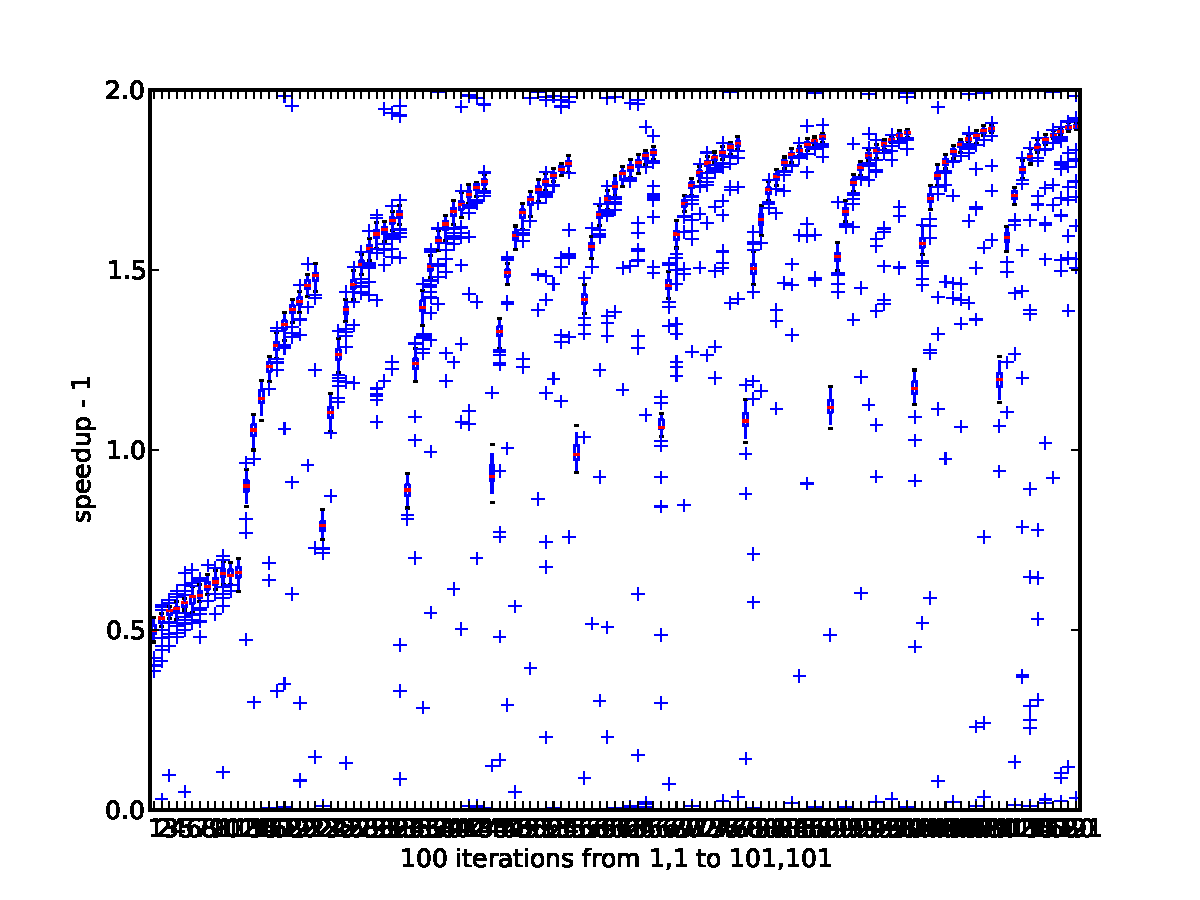
\includegraphics[scale=0.25]{images/openmp_measures_for_2_cores_n1_no_vartime_1_speedup_p1_pS10_P101_d1_dS10_D101_r100_s1.pdf}}
\subfloat[dynamicité sur 2 coeurs]{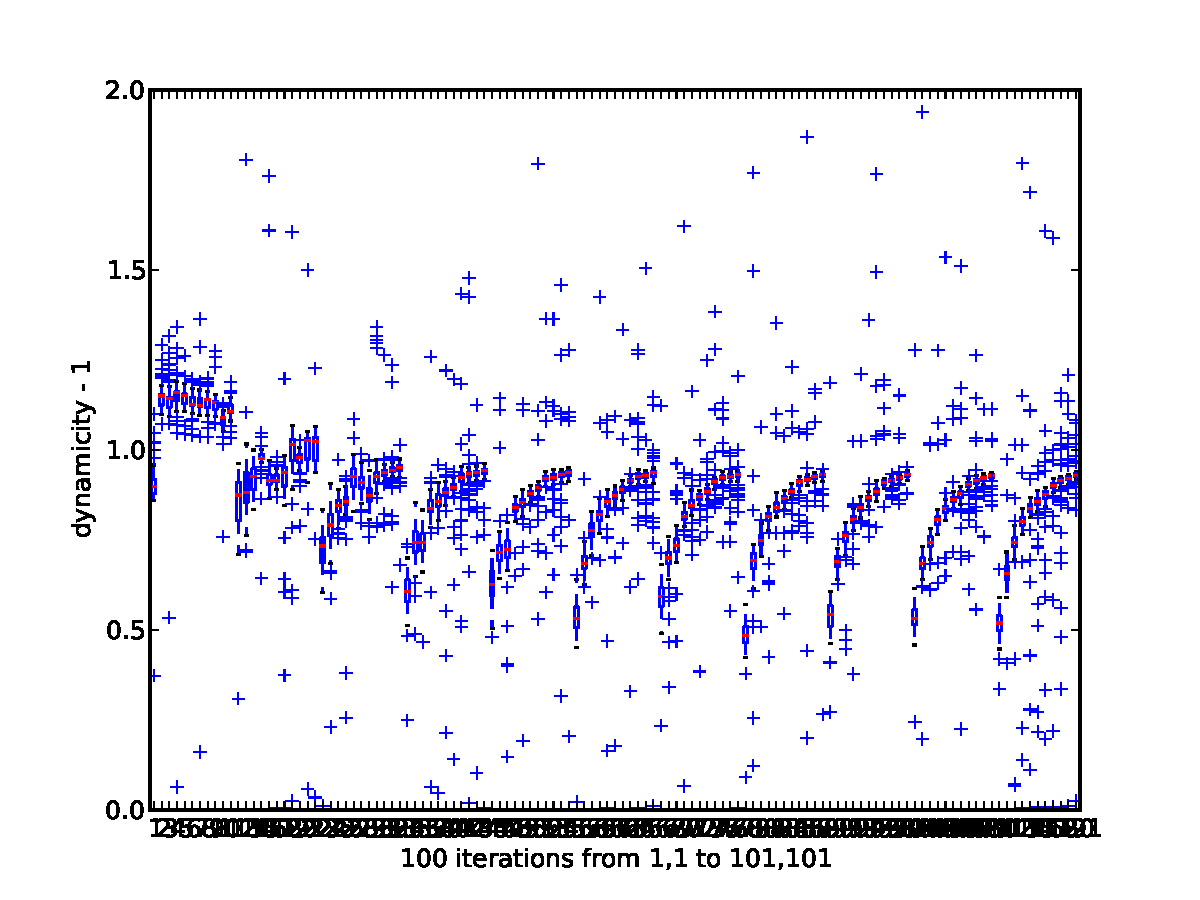
\includegraphics[scale=0.25]{images/openmp_measures_for_2_cores_n1_no_vartime_1_dynamicity_p1_pS10_P101_d1_dS10_D101_r100_s1.pdf}}
\qquad
\subfloat[speedup sur 8 coeurs]{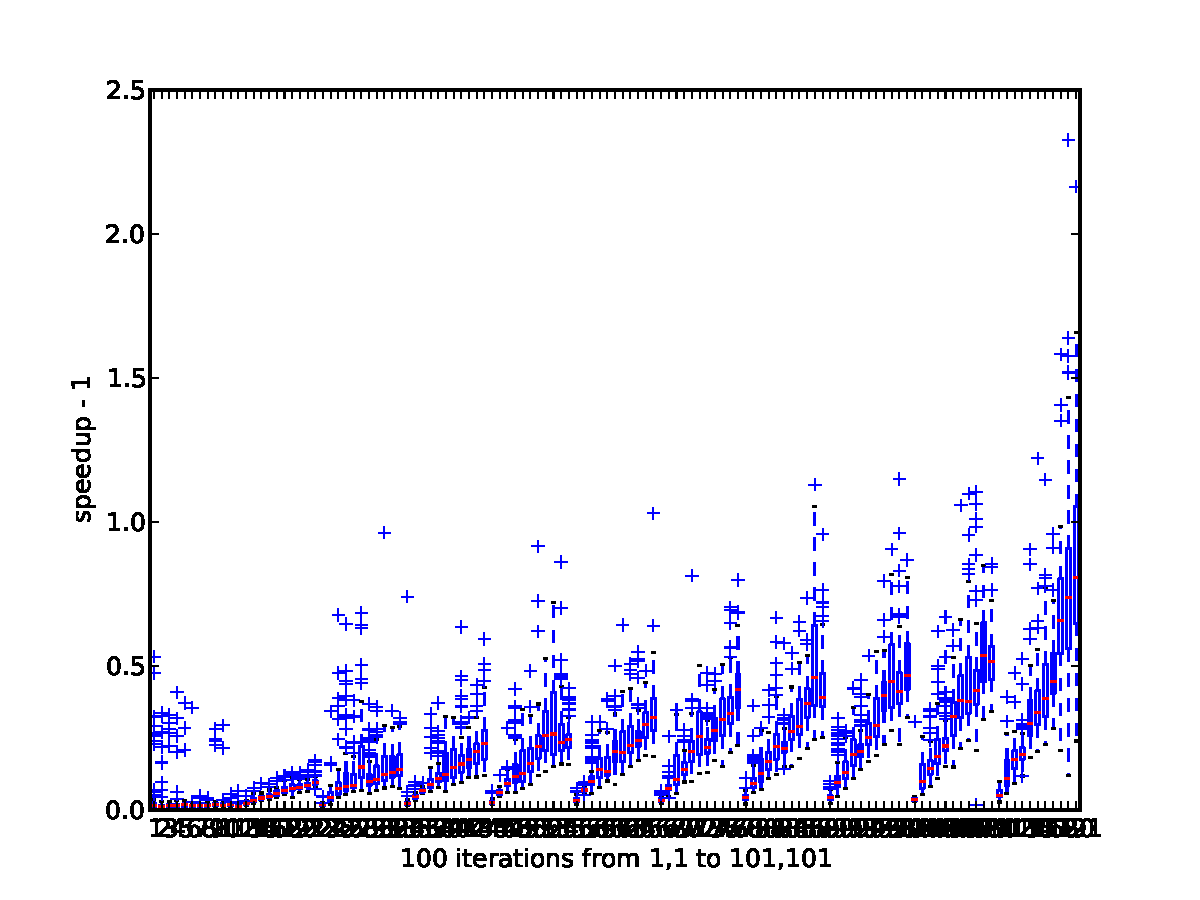
\includegraphics[scale=0.25]{images/openmp_measures_for_8_cores_n1_no_vartime_1_speedup_p1_pS10_P101_d1_dS10_D101_r100_s1.pdf}}
\subfloat[dynamicité sur 8 coeurs]{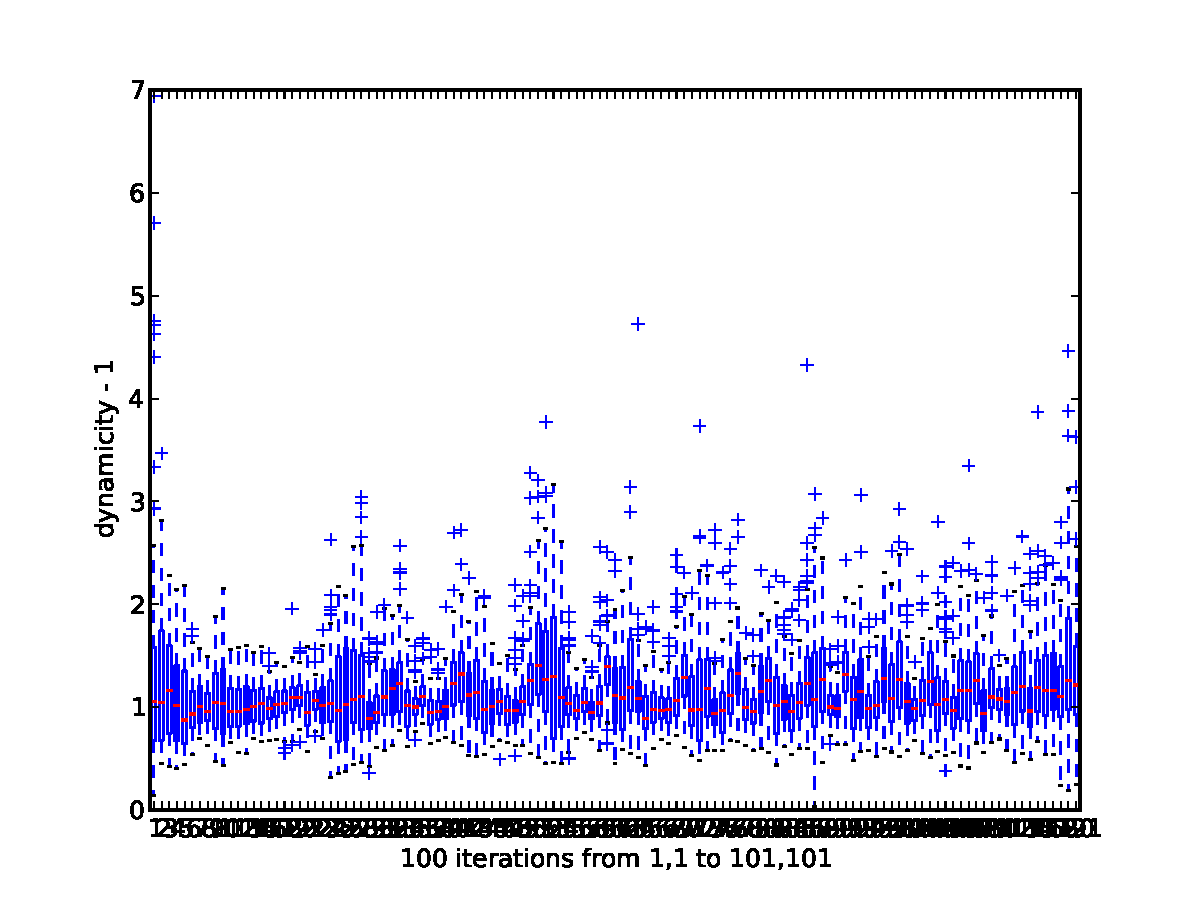
\includegraphics[scale=0.25]{images/openmp_measures_for_8_cores_n1_no_vartime_1_dynamicity_p1_pS10_P101_d1_dS10_D101_r100_s1.pdf}}
\caption{Mesure 1 en $O(1)$ sur 2 et 8 coeurs}
\label{fig:mesure_1_constant}
\end{figure}

% mesure 2 en O(1)
\begin{figure}[here]
\centering
\subfloat[speedup sur 2 coeurs]{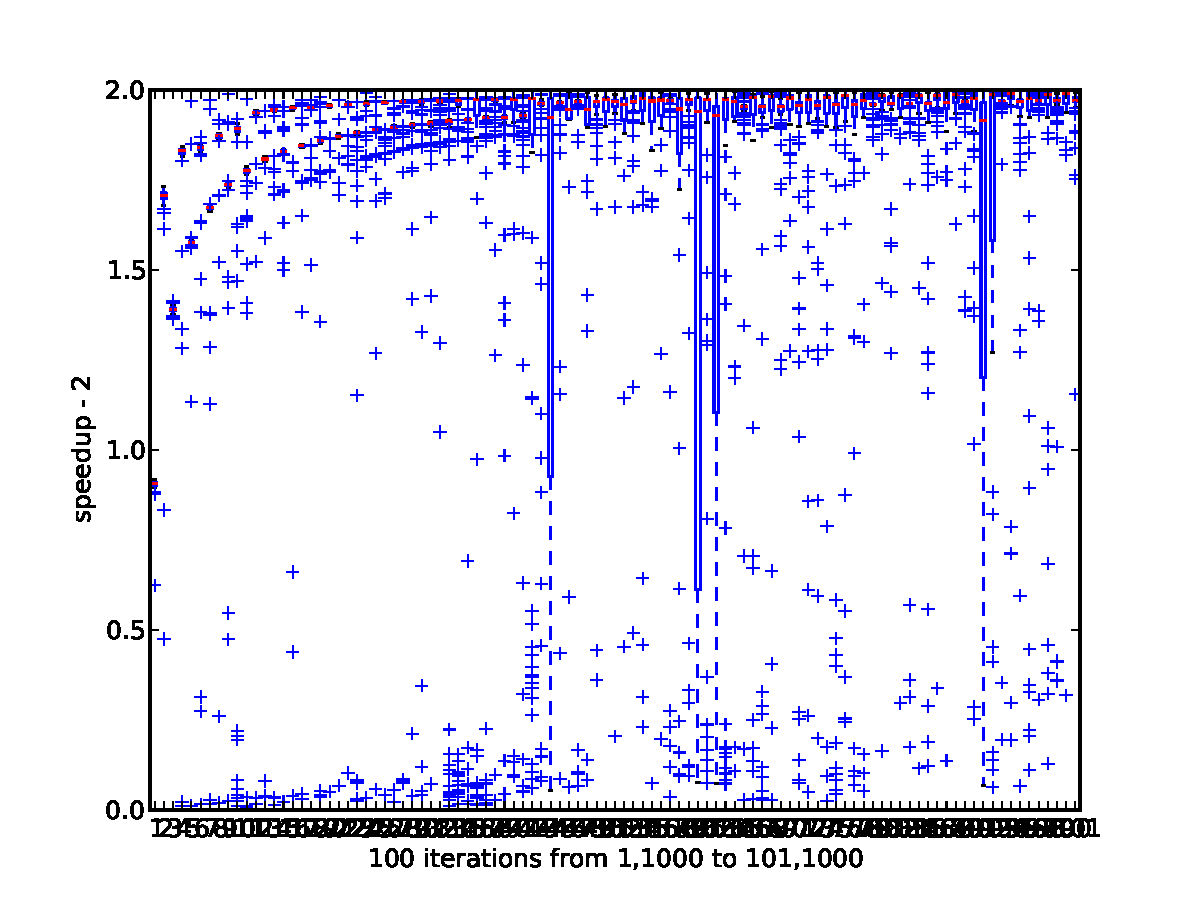
\includegraphics[scale=0.25]{images/openmp_measures_for_2_cores_n1_no_vartime_2_speedup_p1_pS1_P101_d1000_dS1_D1000_r100_s1.pdf}}
\subfloat[dynamicité sur 2 coeurs]{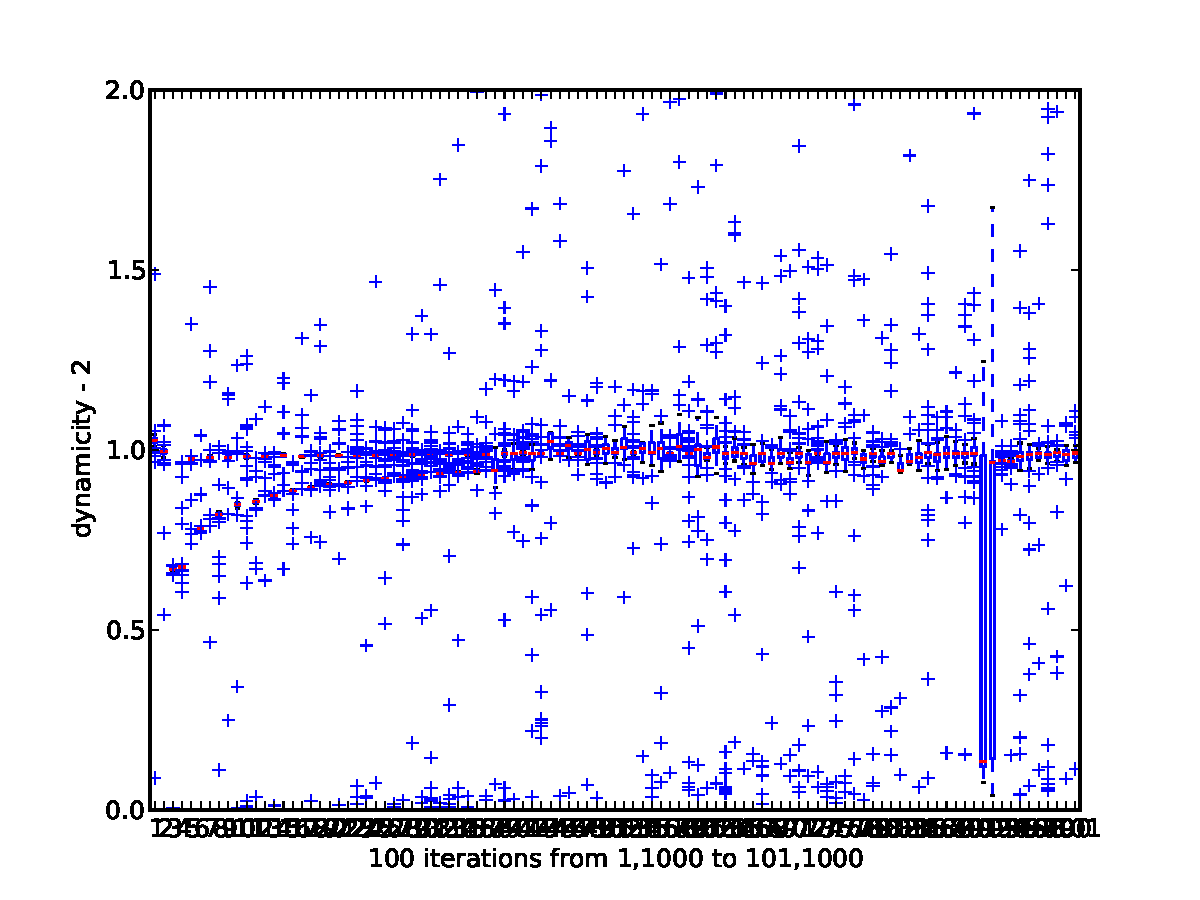
\includegraphics[scale=0.25]{images/openmp_measures_for_2_cores_n1_no_vartime_2_dynamicity_p1_pS1_P101_d1000_dS1_D1000_r100_s1.pdf}}
\qquad
\subfloat[speedup sur 8 coeurs]{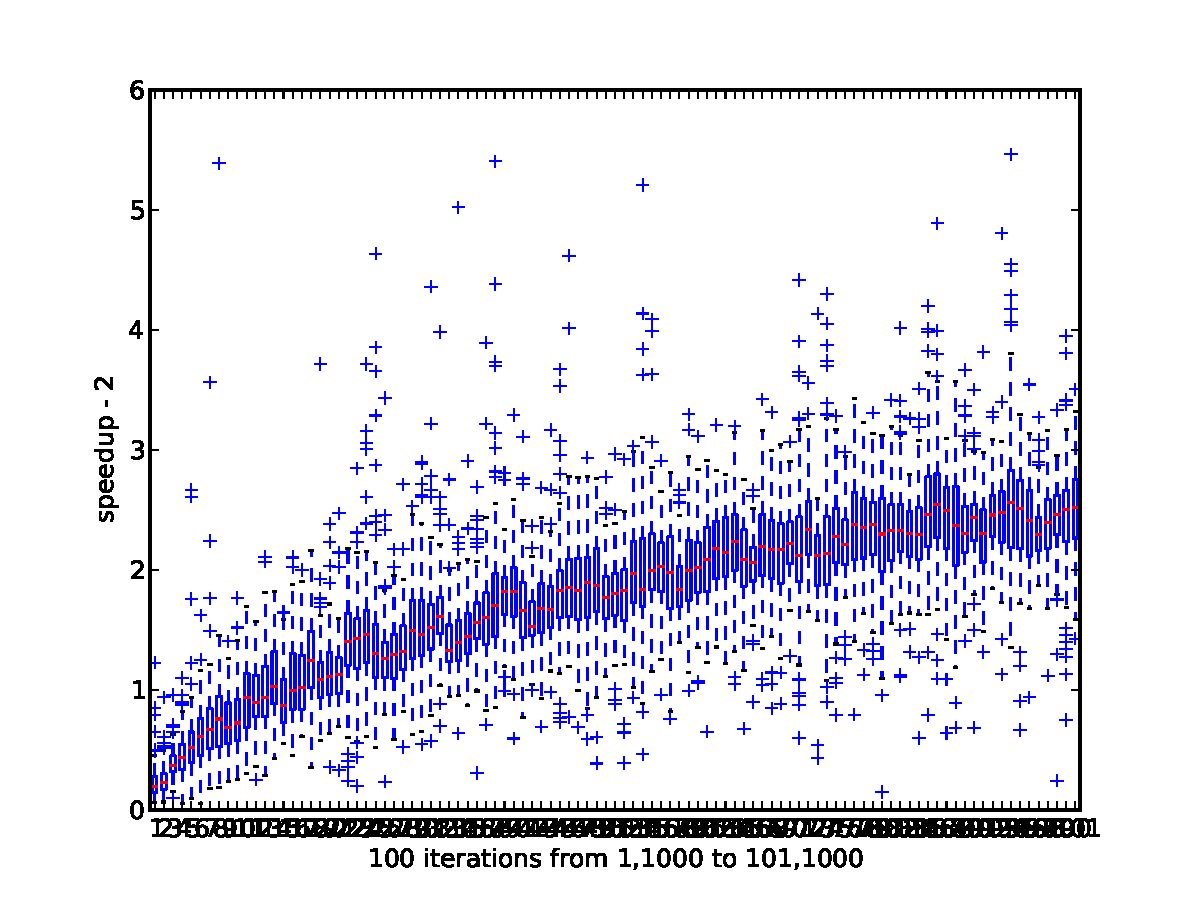
\includegraphics[scale=0.25]{images/openmp_measures_for_8_cores_n1_no_vartime_2_speedup_p1_pS1_P101_d1000_dS1_D1000_r100_s1.pdf}}
\subfloat[dynamicité sur 8 coeurs]{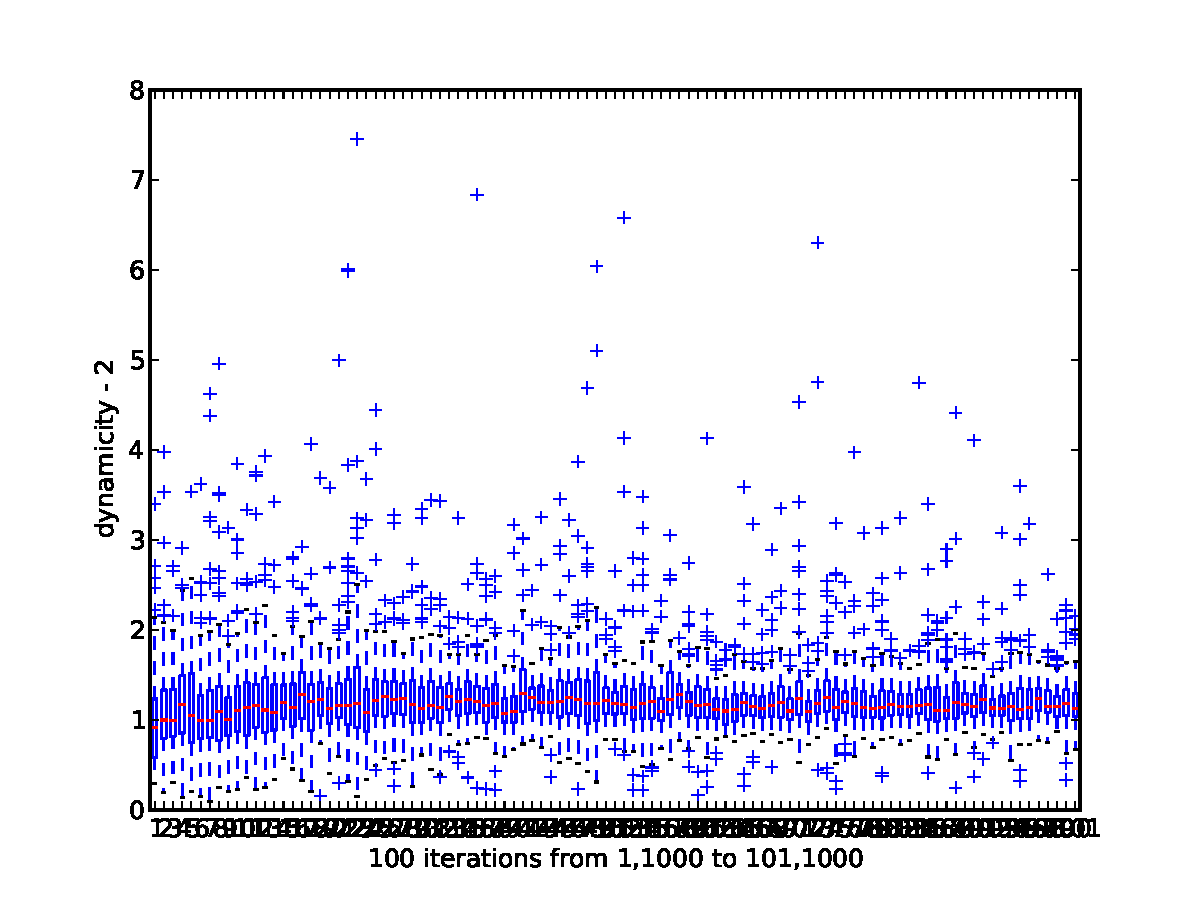
\includegraphics[scale=0.25]{images/openmp_measures_for_8_cores_n1_no_vartime_2_dynamicity_p1_pS1_P101_d1000_dS1_D1000_r100_s1.pdf}}
\caption{Mesure 2 en $O(1)$ sur 2 et 8 coeurs}
\label{fig:mesure_2_constant}
\end{figure}

% mesure 3 en O(1)
\begin{figure}[here]
\centering
\subfloat[speedup sur 2 coeurs]{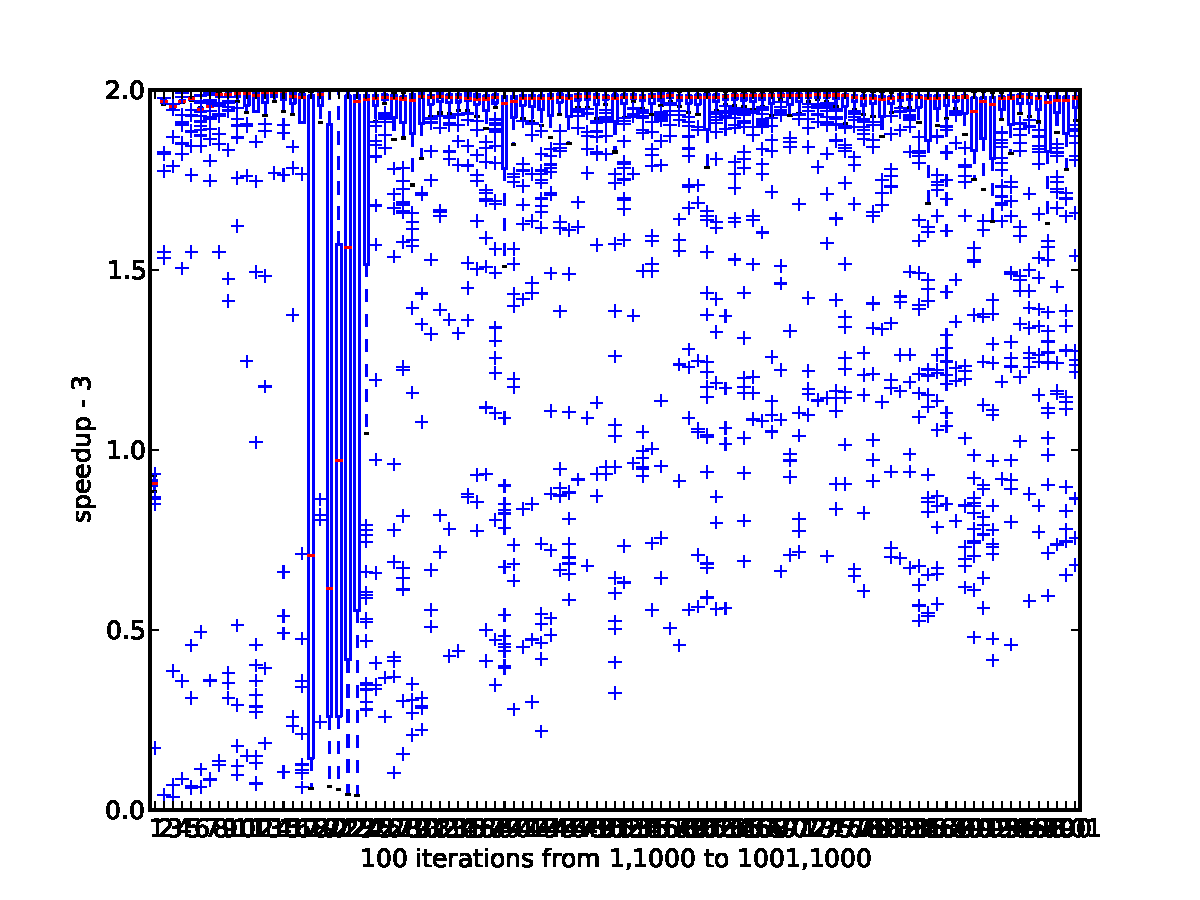
\includegraphics[scale=0.25]{images/openmp_measures_for_2_cores_n1_no_vartime_3_speedup_p1_pS10_P1001_d1000_dS1_D1000_r100_s1.pdf}}
\subfloat[dynamicité sur 2 coeurs]{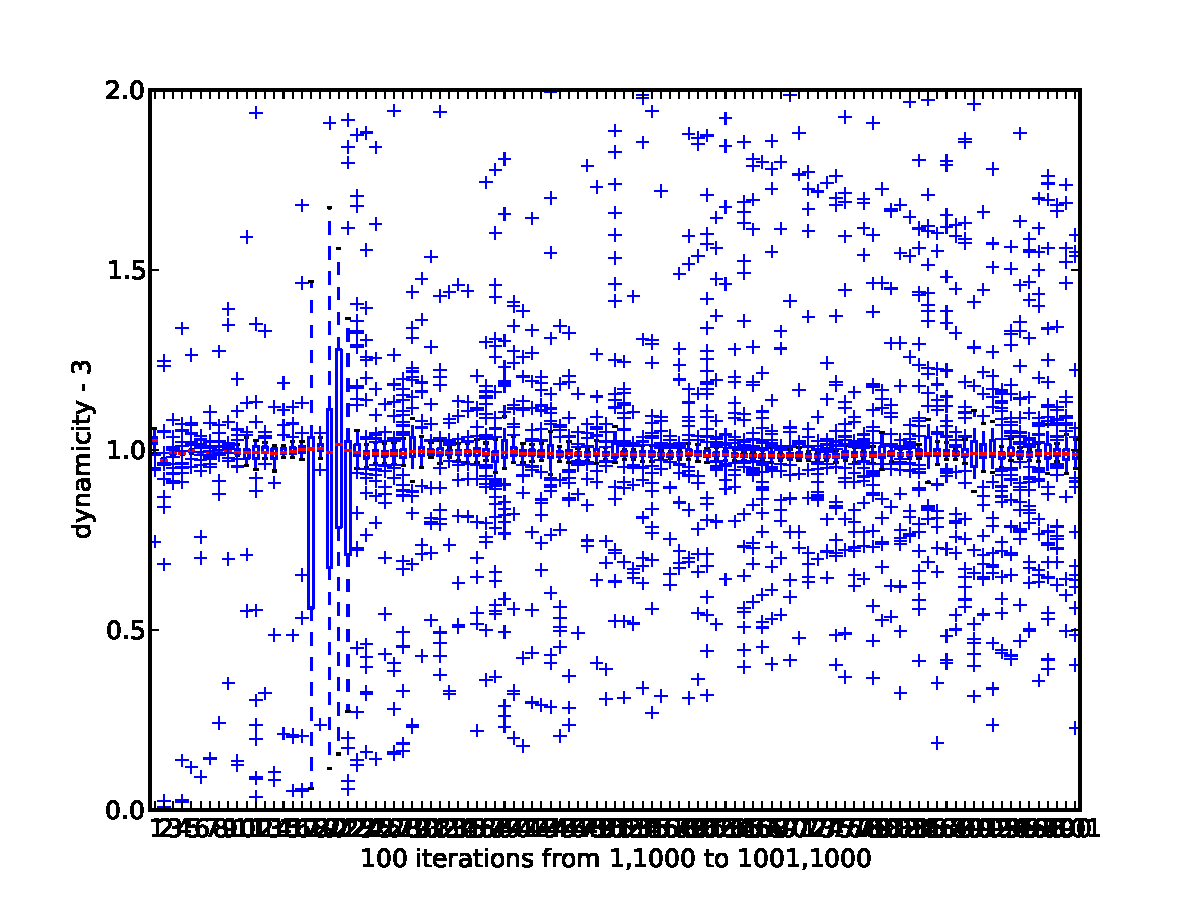
\includegraphics[scale=0.25]{images/openmp_measures_for_2_cores_n1_no_vartime_3_dynamicity_p1_pS10_P1001_d1000_dS1_D1000_r100_s1.pdf}}
\qquad
\subfloat[speedup sur 8 coeurs]{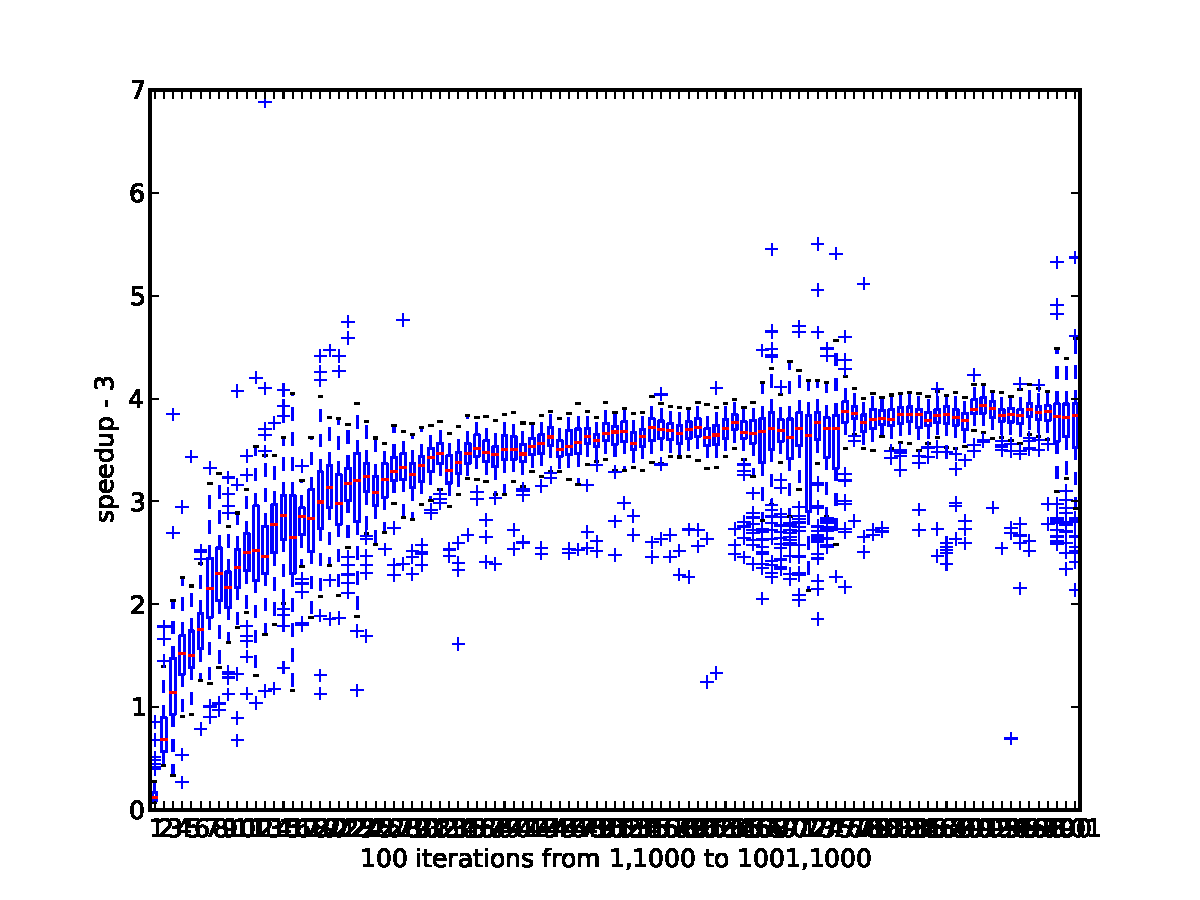
\includegraphics[scale=0.25]{images/openmp_measures_for_8_cores_n1_no_vartime_3_speedup_p1_pS10_P1001_d1000_dS1_D1000_r100_s1.pdf}}
\subfloat[dynamicité sur 8 coeurs]{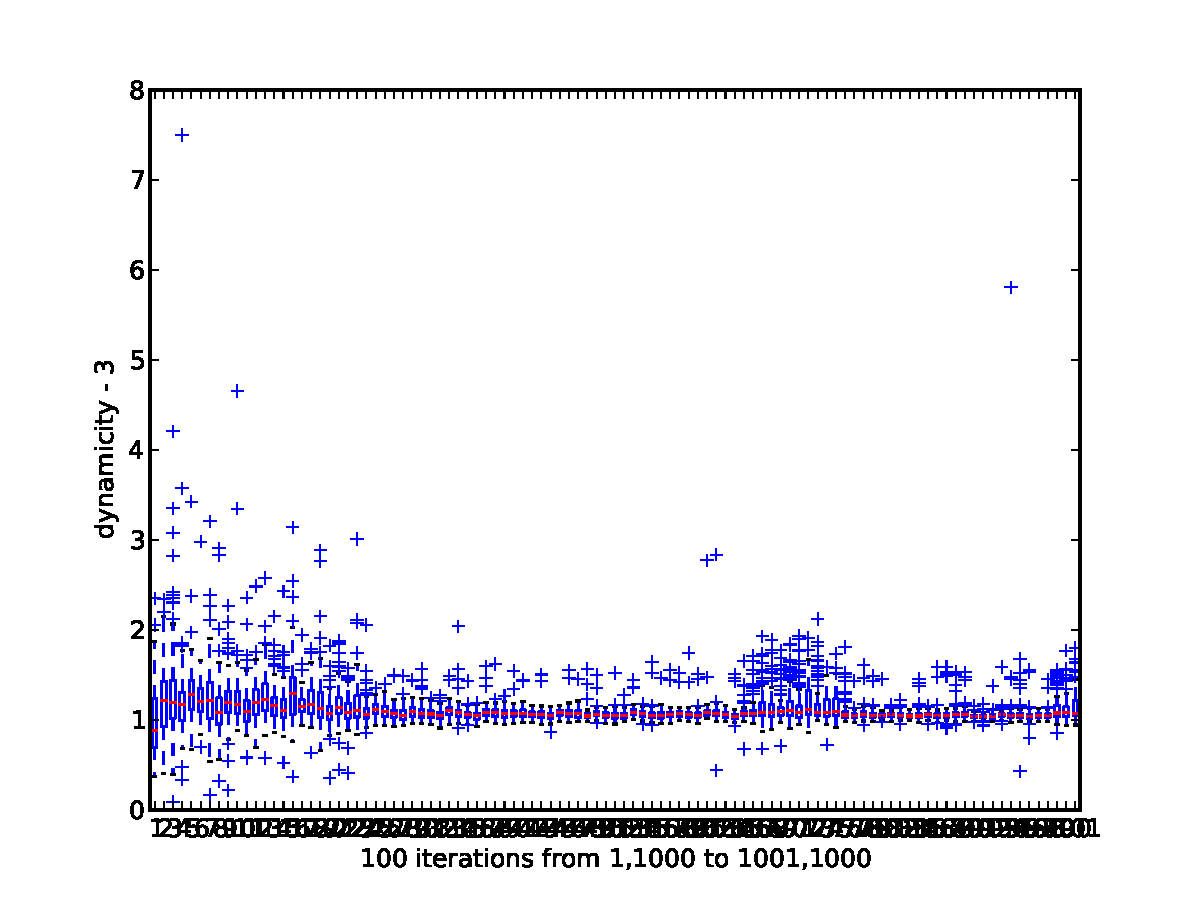
\includegraphics[scale=0.25]{images/openmp_measures_for_8_cores_n1_no_vartime_3_dynamicity_p1_pS10_P1001_d1000_dS1_D1000_r100_s1.pdf}}
\caption{Mesure 3 en $O(1)$ sur 2 et 8 coeurs}
\label{fig:mesure_3_constant}
\end{figure}

% mesure 4 en O(1)
\begin{figure}[here]
\centering
\subfloat[speedup sur 2 coeurs]{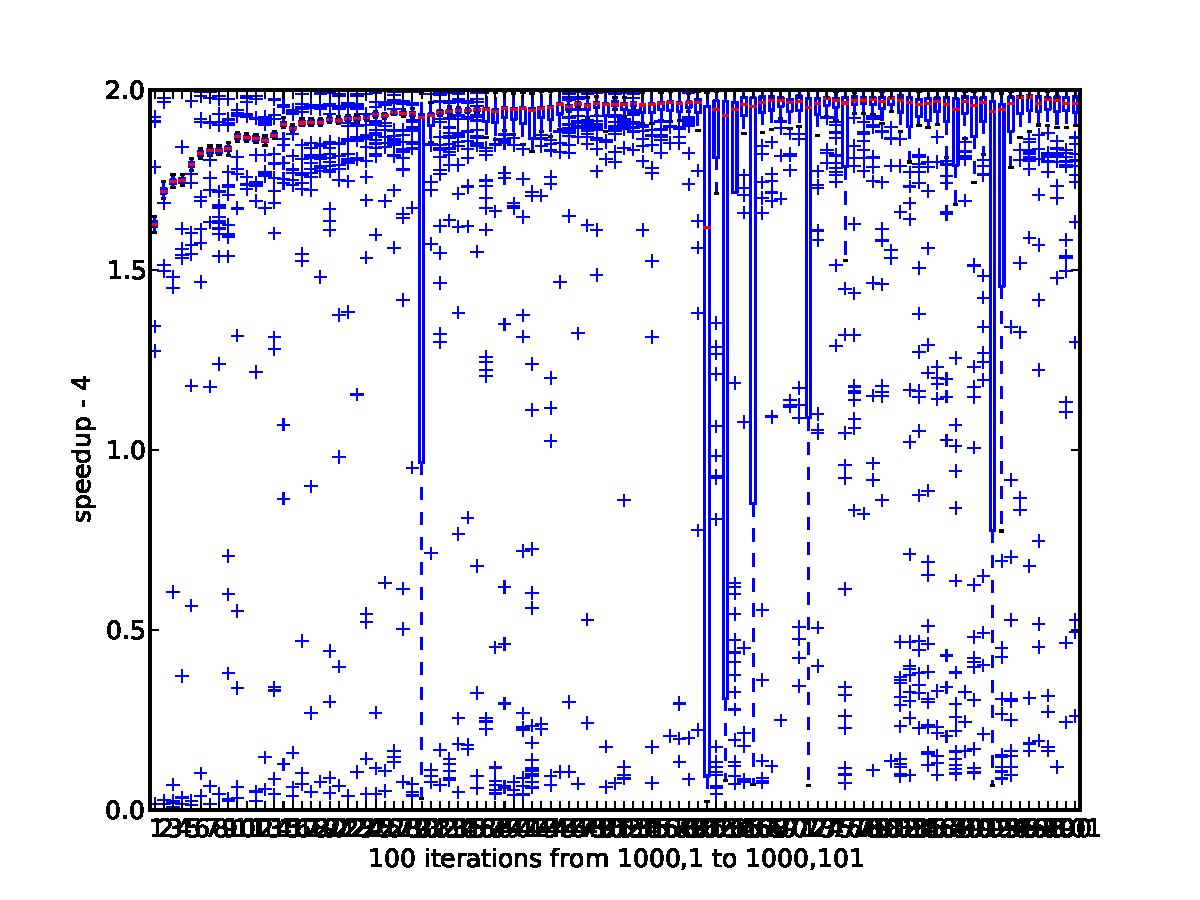
\includegraphics[scale=0.25]{images/openmp_measures_for_2_cores_n1_no_vartime_4_speedup_p1000_pS1_P1000_d1_dS1_D101_r100_s1.pdf}}
\subfloat[dynamicité sur 2 coeurs]{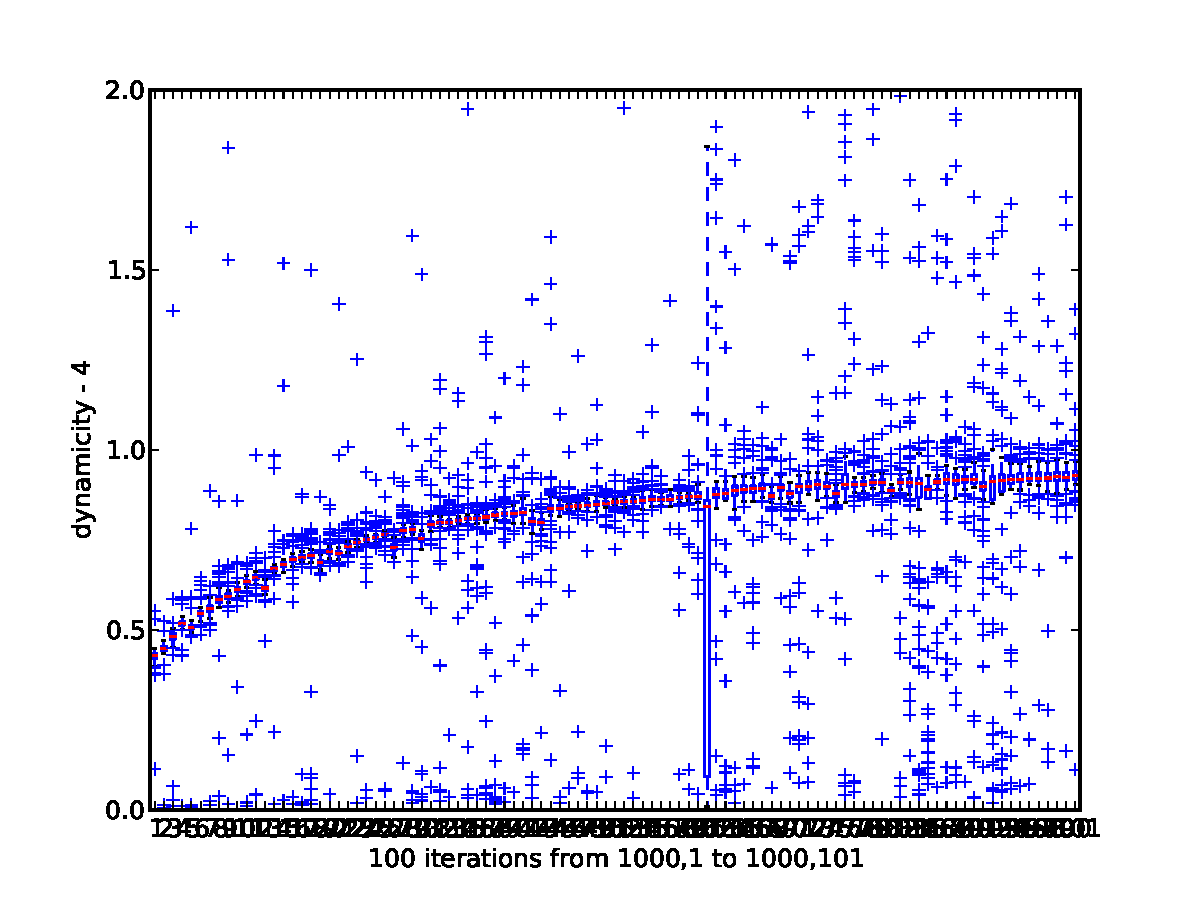
\includegraphics[scale=0.25]{images/openmp_measures_for_2_cores_n1_no_vartime_4_dynamicity_p1000_pS1_P1000_d1_dS1_D101_r100_s1.pdf}}
\qquad
\subfloat[speedup sur 8 coeurs]{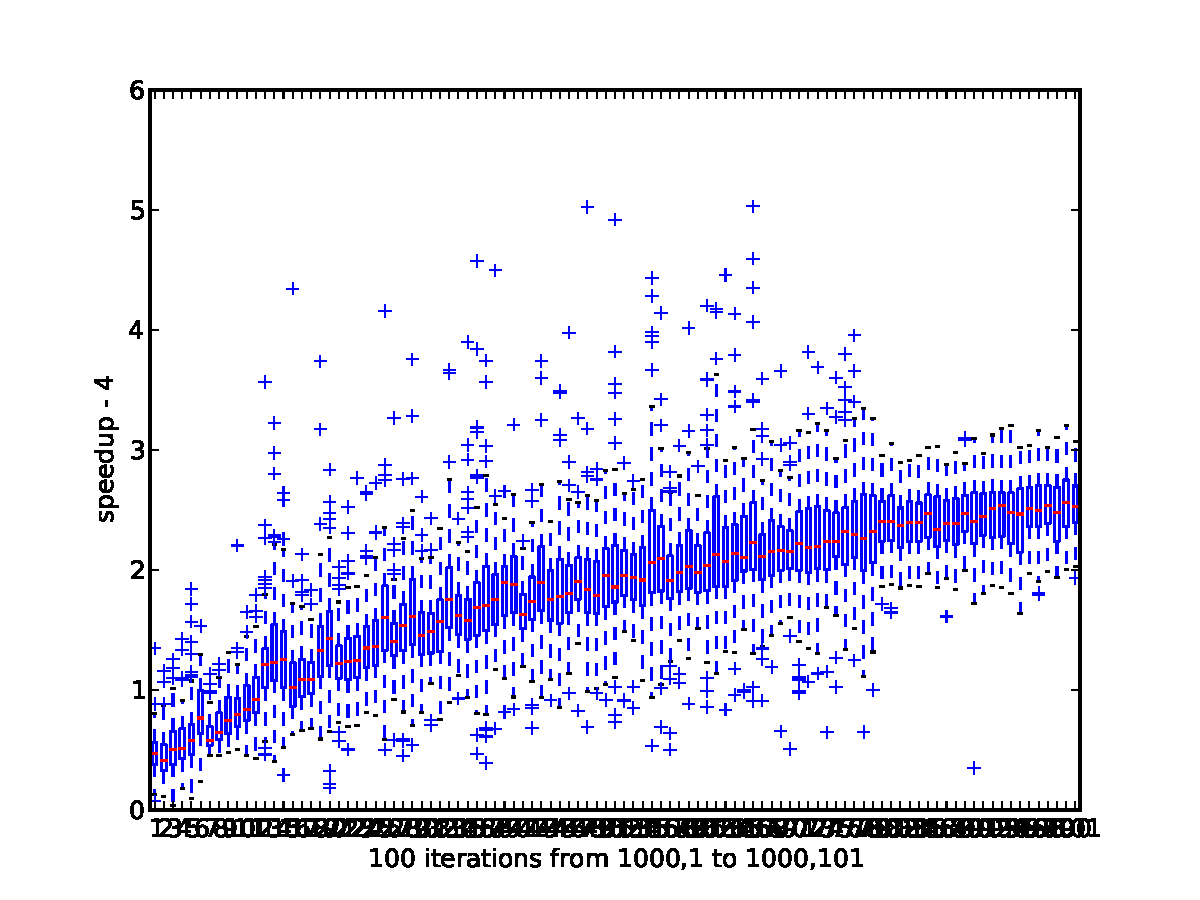
\includegraphics[scale=0.25]{images/openmp_measures_for_8_cores_n1_no_vartime_4_speedup_p1000_pS1_P1000_d1_dS1_D101_r100_s1.pdf}}
\subfloat[dynamicité sur 8 coeurs]{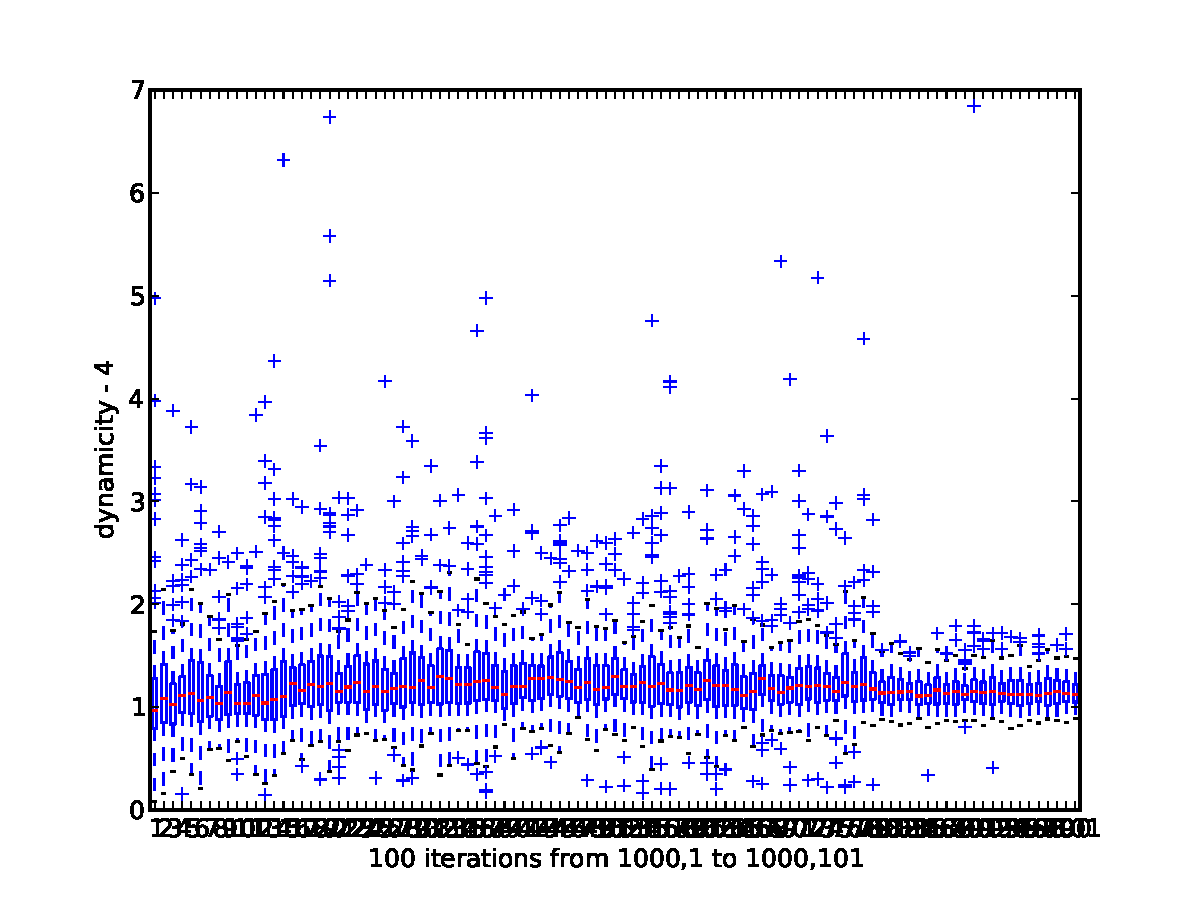
\includegraphics[scale=0.25]{images/openmp_measures_for_8_cores_n1_no_vartime_4_dynamicity_p1000_pS1_P1000_d1_dS1_D101_r100_s1.pdf}}
\caption{Mesure 4 en $O(1)$ sur 2 et 8 coeurs}
\label{fig:mesure_4_constant}
\end{figure}

% mesure 5 en O(1)
\begin{figure}[here]
\centering
\subfloat[speedup sur 2 coeurs]{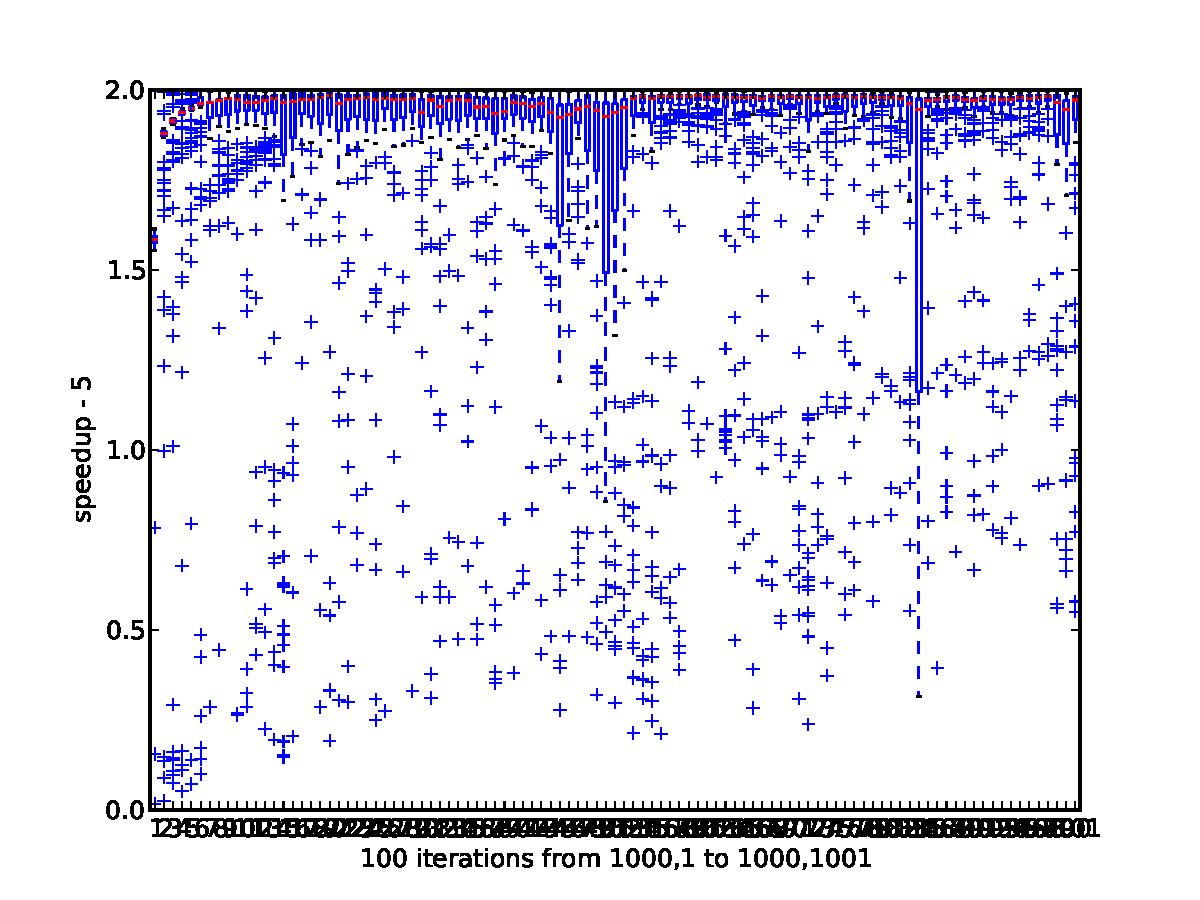
\includegraphics[scale=0.25]{images/openmp_measures_for_2_cores_n1_no_vartime_5_speedup_p1000_pS1_P1000_d1_dS10_D1001_r100_s1.pdf}}
\subfloat[dynamicité sur 2 coeurs]{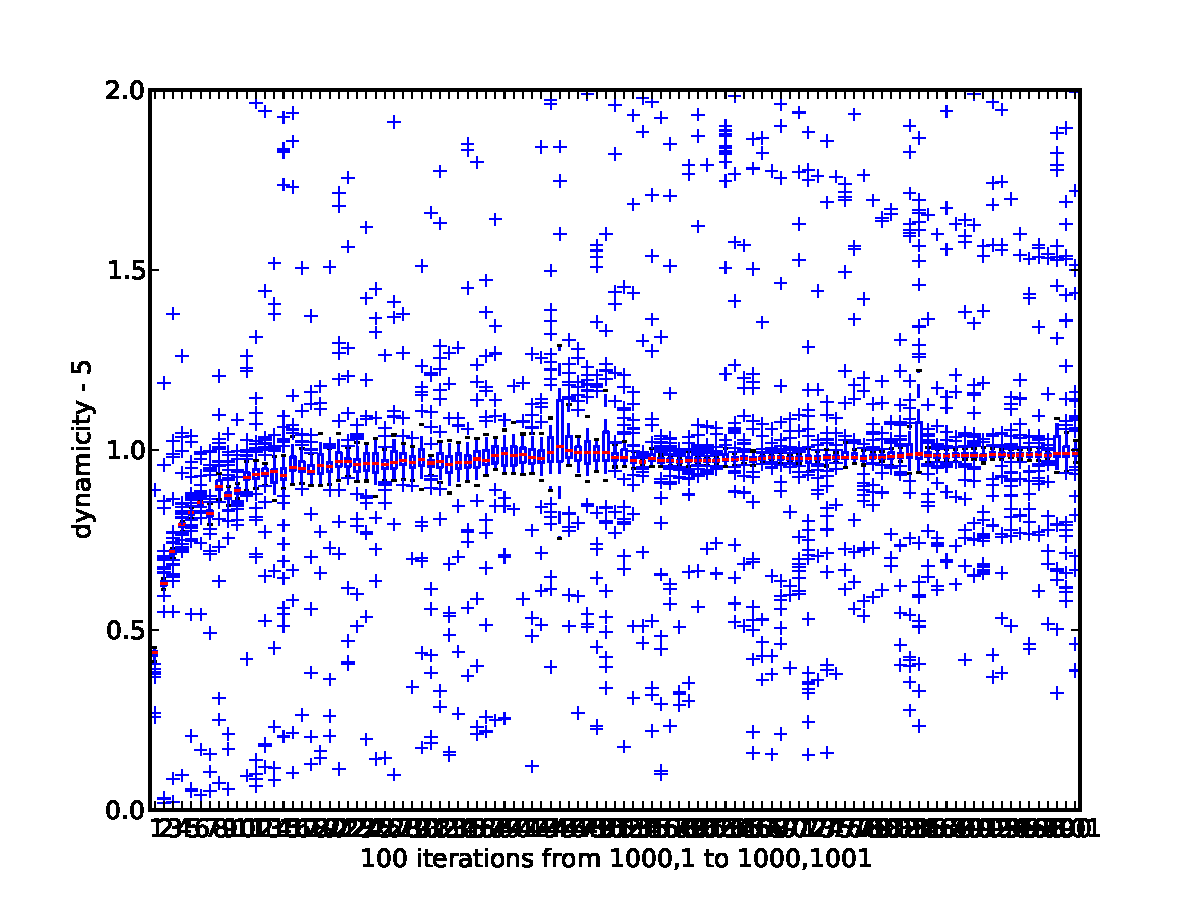
\includegraphics[scale=0.25]{images/openmp_measures_for_2_cores_n1_no_vartime_5_dynamicity_p1000_pS1_P1000_d1_dS10_D1001_r100_s1.pdf}}
\qquad
\subfloat[speedup sur 8 coeurs]{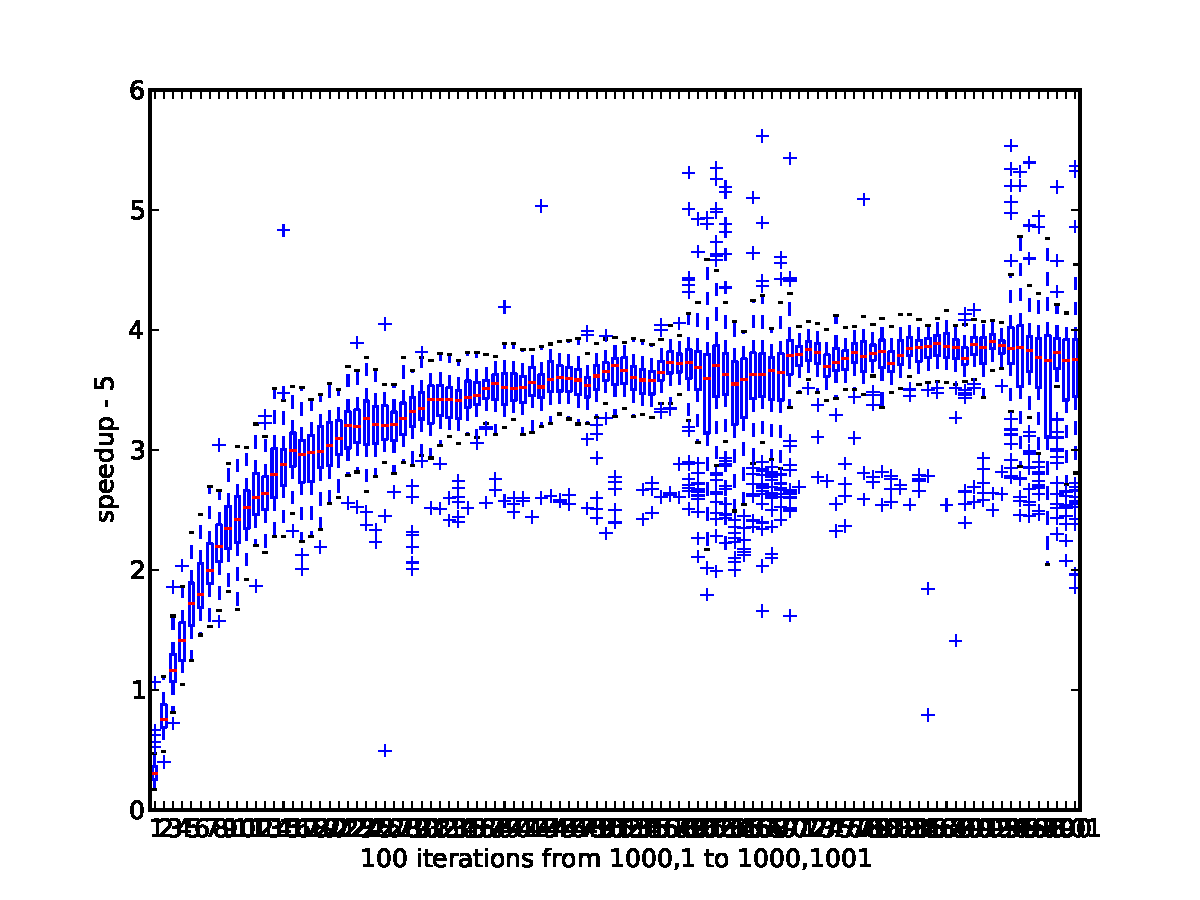
\includegraphics[scale=0.25]{images/openmp_measures_for_8_cores_n1_no_vartime_5_speedup_p1000_pS1_P1000_d1_dS10_D1001_r100_s1.pdf}}
\subfloat[dynamicité sur 8 coeurs]{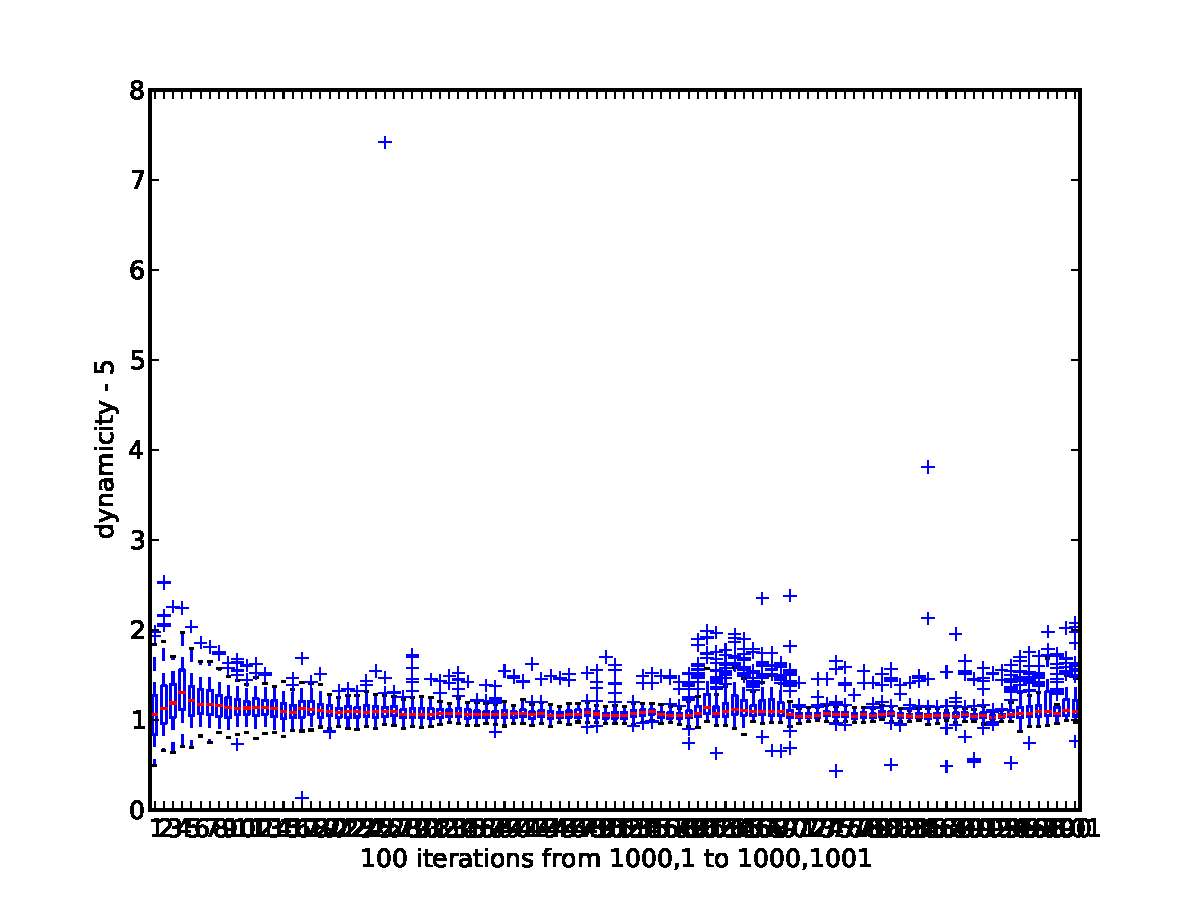
\includegraphics[scale=0.25]{images/openmp_measures_for_8_cores_n1_no_vartime_5_dynamicity_p1000_pS1_P1000_d1_dS10_D1001_r100_s1.pdf}}
\caption{Mesure 5 en $O(1)$ sur 2 et 8 coeurs}
\label{fig:mesure_5_constant}
\end{figure}

\newpage

\subsubsection{Résultats en $O(n)$}

Dans un second temps, le benchmark est exécuté pour le problème qui se résoud en temps variable. Les résultats de chaque mesure sont numérotés d'après le tableau des mesures décrit précédemment en figure \ref{fig:liste_mesures}.\\

Il est important d'ajouter que compte tenu de la résolution du problème en $O(n)$ et non plus en fonction de la dimension, celle ci perd de son importance. Ainsi les mesures 1, 4 et 5 ne sont plus nessaire à mesurer. Seules les mesures 2 et 3 seront présentées ci-dessous.\\

Un algorithme séquentiel exécuté sur un processeur à 8 coeurs en comparaison avec un processeur à 2 coeurs est plus performant sur des petits échantillons. Nous avons donc choisit de définir les bornes des paramètres, décrits en figure \ref{fig:liste_mesures}, comme multiple du nombre de coeurs disponible.\\

Les mesures sont présentées en fonction des processeurs utilisés et disponibles en figure \ref{fig:mesure_2_variable} et \ref{fig:mesure_3_variable}.

% mesure 2 en O(n)
\begin{figure}[here]
\centering
\subfloat[speedup sur 2 coeurs]{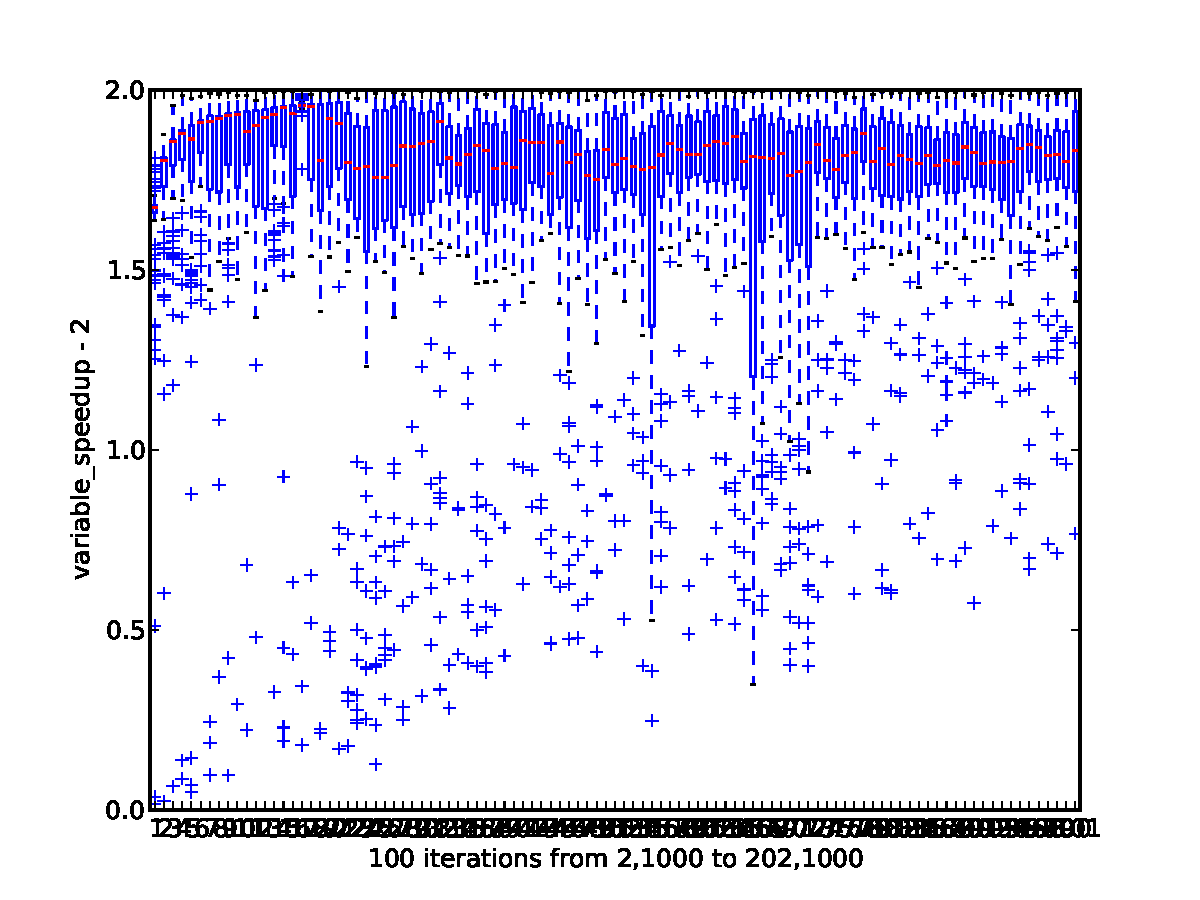
\includegraphics[scale=0.25]{images/openmp_measures_for_2_cores_n2_2_variable_speedup_p2_pS2_P202_d1000_dS1_D1000_r100_s1.pdf}}
\subfloat[dynamicité sur 2 coeurs]{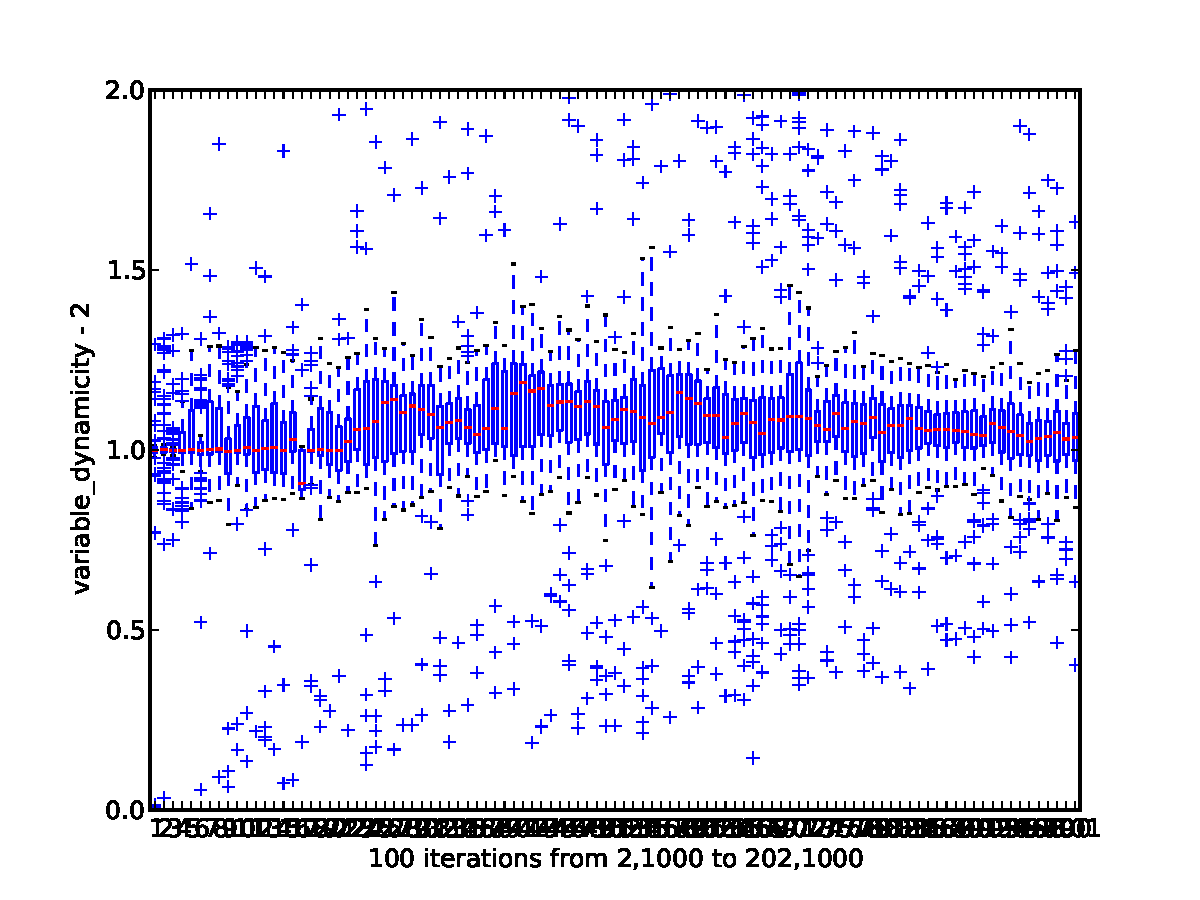
\includegraphics[scale=0.25]{images/openmp_measures_for_2_cores_n2_2_variable_dynamicity_p2_pS2_P202_d1000_dS1_D1000_r100_s1.pdf}}
\qquad
\subfloat[speedup sur 8 coeurs]{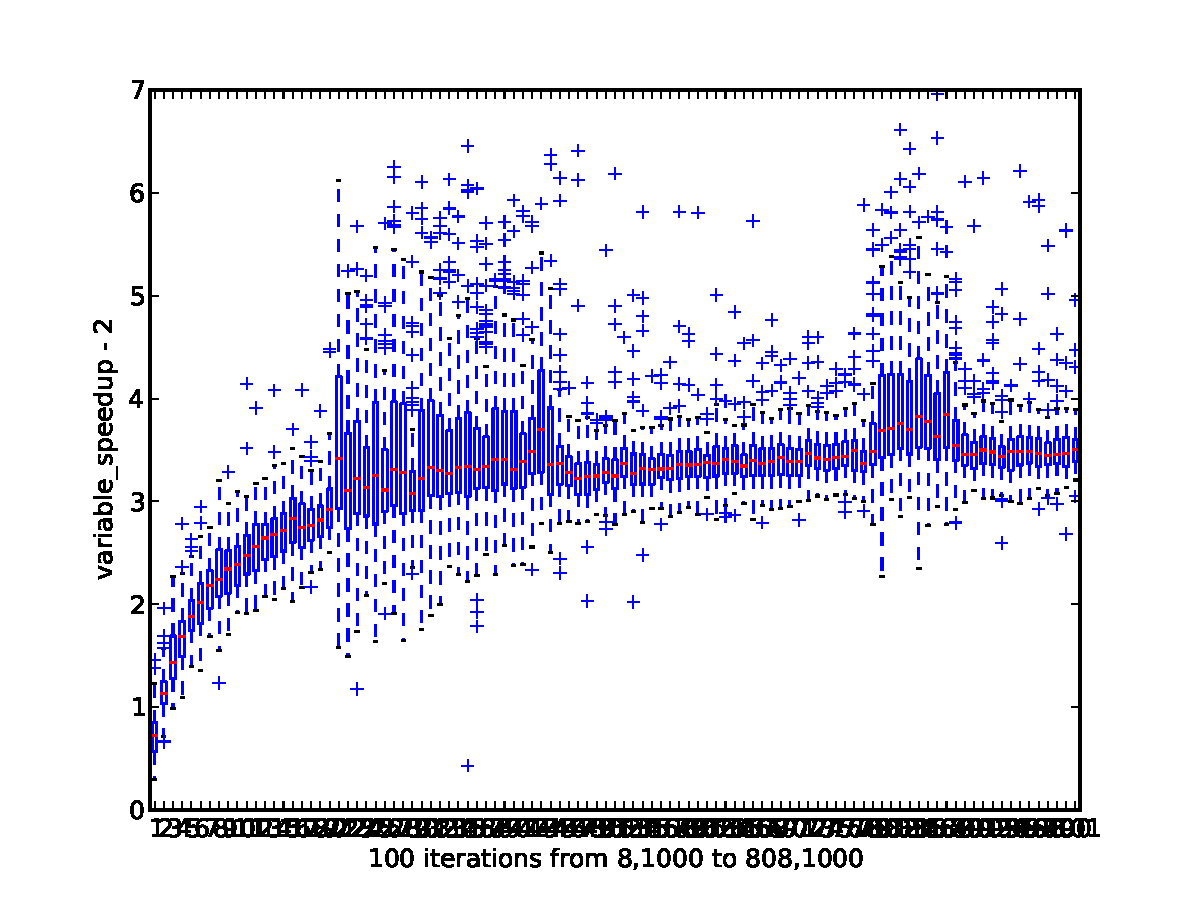
\includegraphics[scale=0.25]{images/openmp_measures_for_8_cores_n8_no_consttime_2_variable_speedup_p8_pS8_P808_d1000_dS1_D1000_r100_s1.pdf}}
\subfloat[dynamicité sur 8 coeurs]{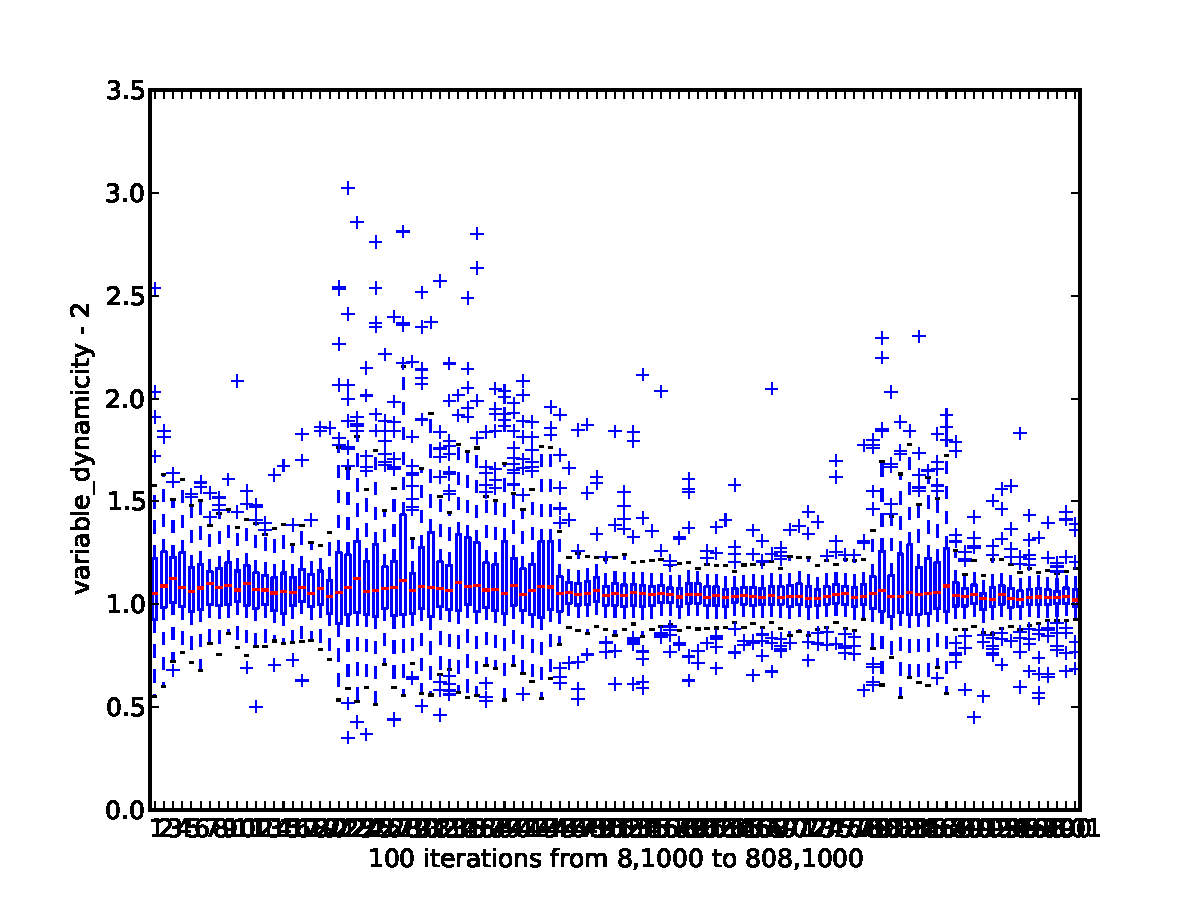
\includegraphics[scale=0.25]{images/openmp_measures_for_8_cores_n8_no_consttime_2_variable_dynamicity_p8_pS8_P808_d1000_dS1_D1000_r100_s1.pdf}}
\caption{Mesure 2 en $O(n)$ sur 2 et 8 coeurs}
\label{fig:mesure_2_variable}
\end{figure}

% mesure 3 en O(1)
\begin{figure}[here]
\centering
\subfloat[speedup sur 2 coeurs]{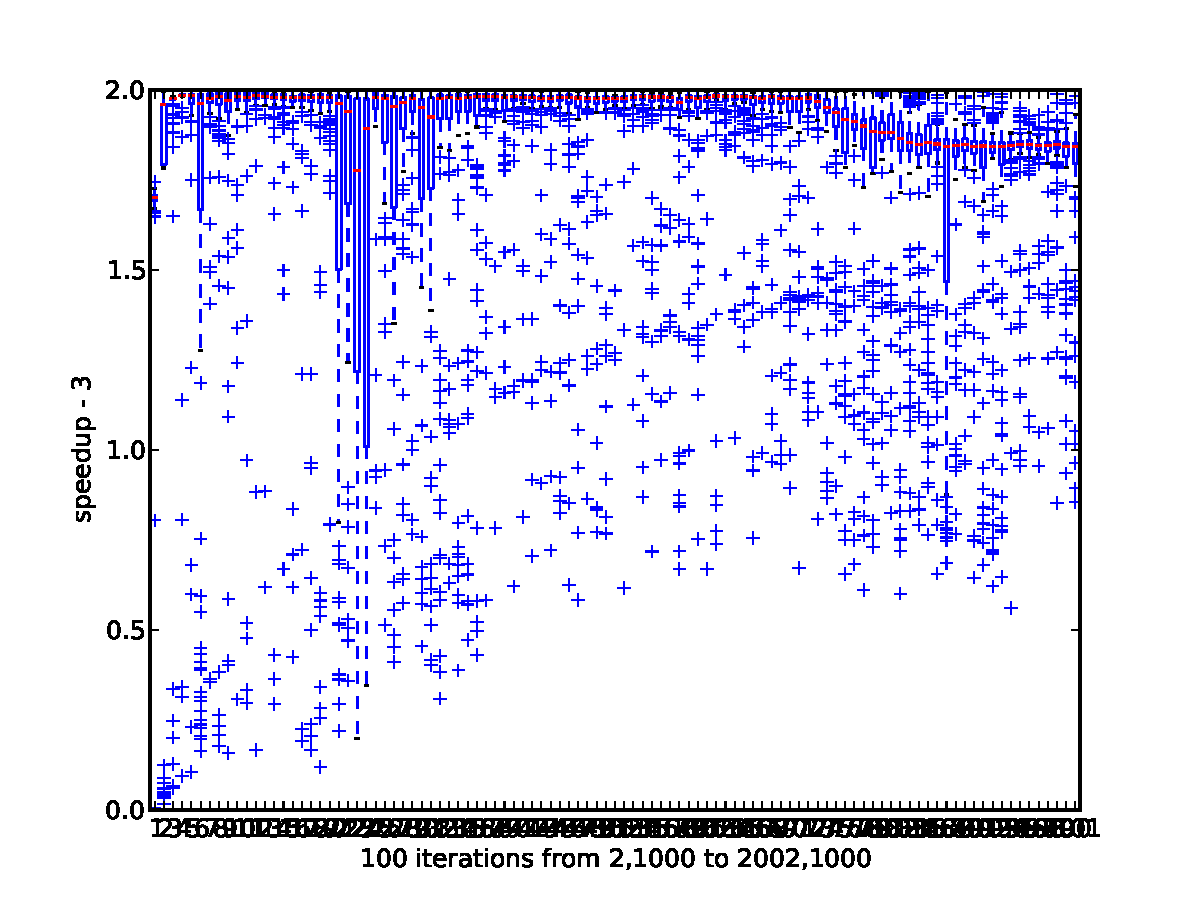
\includegraphics[scale=0.25]{images/openmp_measures_for_2_cores_n2_3_speedup_p2_pS20_P2002_d1000_dS1_D1000_r100_s1.pdf}}
\subfloat[dynamicité sur 2 coeurs]{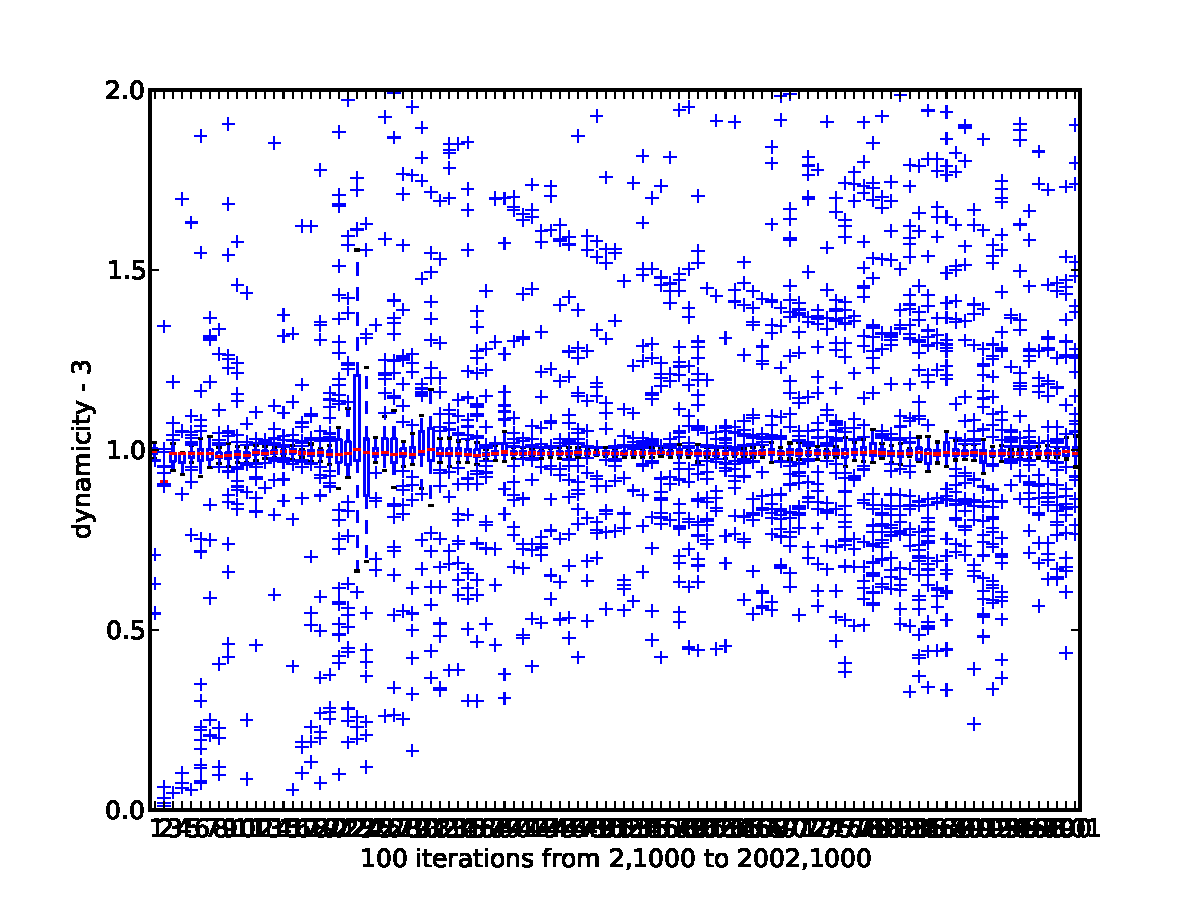
\includegraphics[scale=0.25]{images/openmp_measures_for_2_cores_n2_3_dynamicity_p2_pS20_P2002_d1000_dS1_D1000_r100_s1.pdf}}
\qquad
\subfloat[speedup sur 8 coeurs]{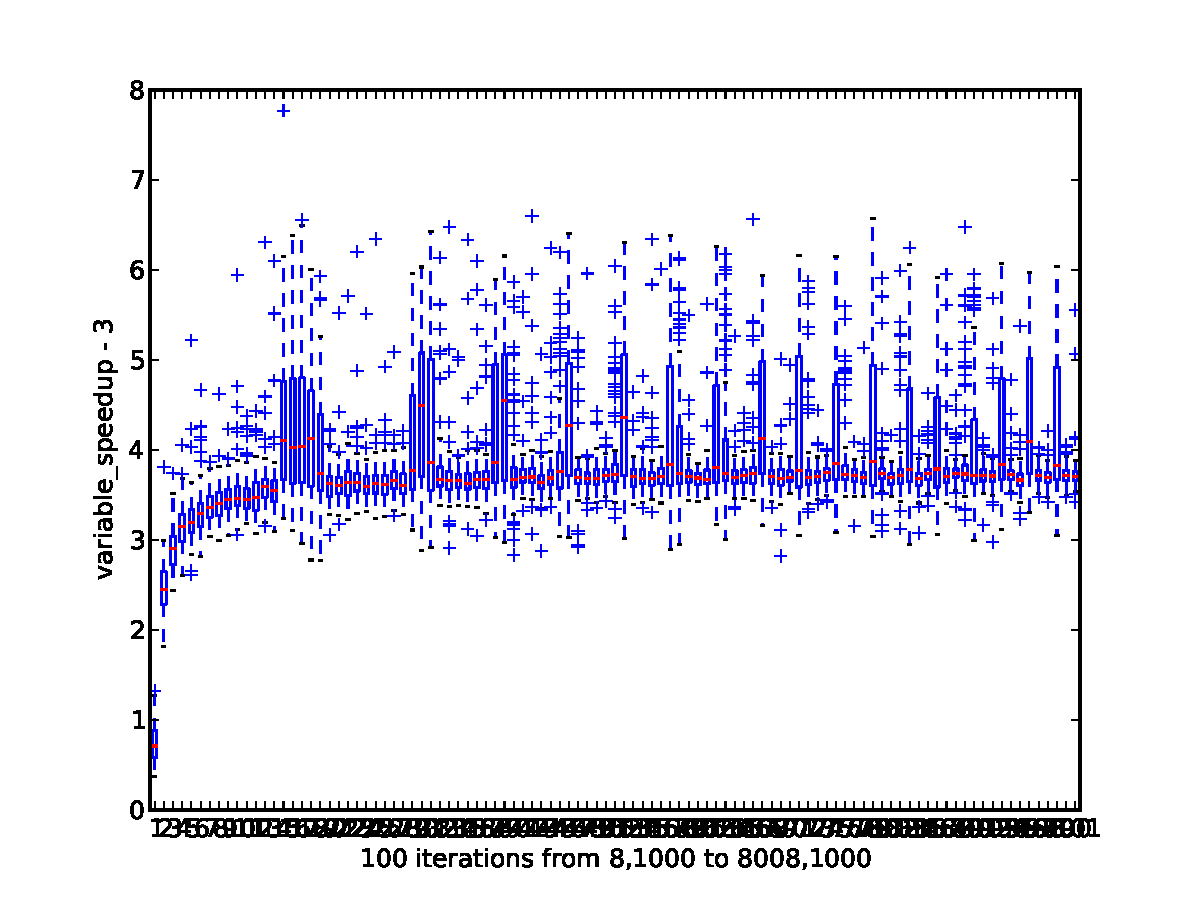
\includegraphics[scale=0.25]{images/openmp_measures_for_8_cores_n8_no_consttime_3_variable_speedup_p8_pS80_P8008_d1000_dS1_D1000_r100_s1.pdf}}
\subfloat[dynamicité sur 8 coeurs]{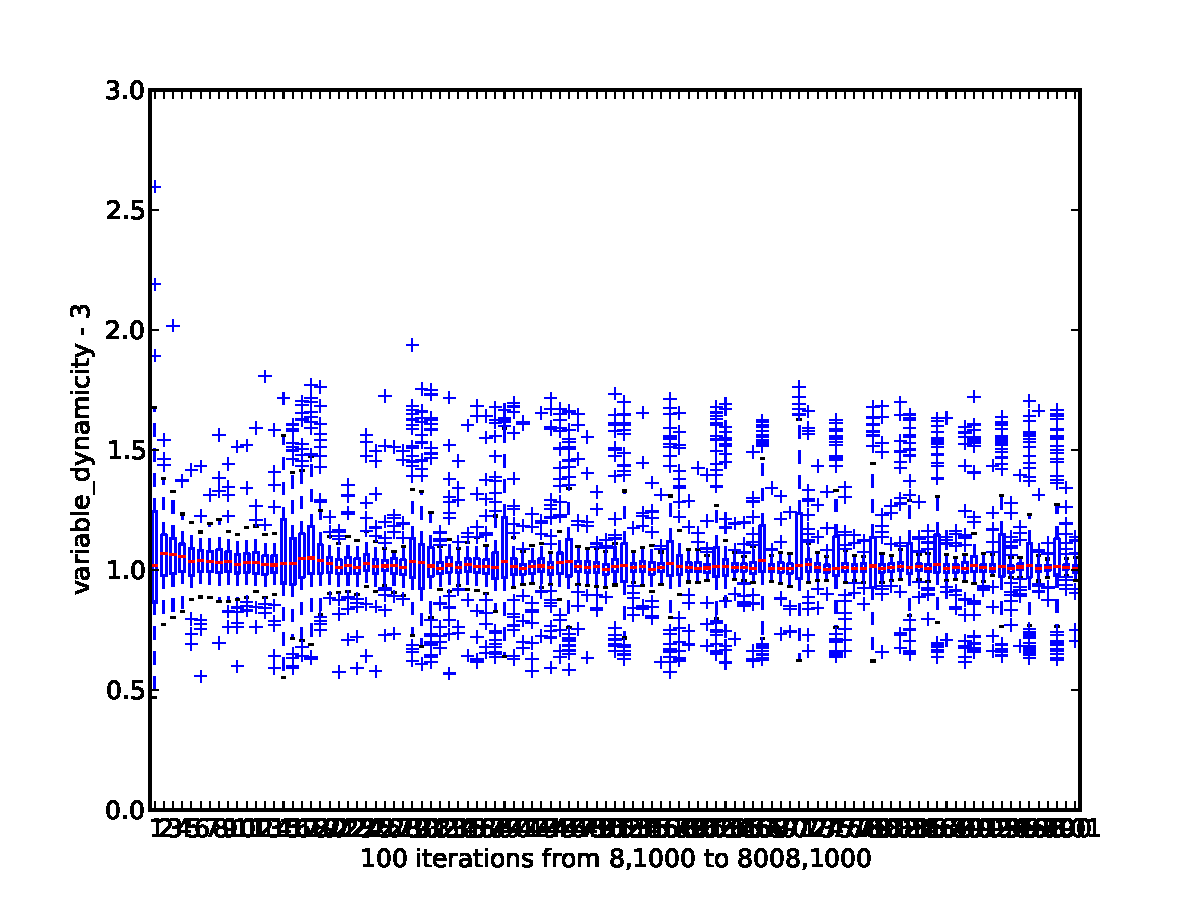
\includegraphics[scale=0.25]{images/openmp_measures_for_8_cores_n8_no_consttime_3_variable_dynamicity_p8_pS80_P8008_d1000_dS1_D1000_r100_s1.pdf}}
\caption{Mesure 3 en $O(n)$ sur 2 et 8 coeurs}
\label{fig:mesure_3_variable}
\end{figure}
